\chapter{Experiments and validation}
\label{chap:validation}

This chapter explains the process of validating each individual piece necessary for the correct operation of the complete system, from testing the first simulation steps to carrying out thorough flight tests on the final guidance solution.
Figure \ref{fig:validation-chart} shows the order in which each step is followed during the validation process.

In the first section, the application is tested in a purely simulated environment, first individually for each part and finally integrating the flight mechanics simulation with providing images to the computer vision detection software and with sending control commands to the flight controller simulation.
In the second section, the follow detection and guidance solution is tested thoroughly to guarantee that only safe velocity commands are outputted from the PID controllers for any image input that could be received and that their response is according to the desired movement of the vehicle.
In the third section, once the software is guaranteed to operate inside the required safety parameters, the simulation is shifted to the dedicated hardware that will be used for actual flight: the dedicated autopilot board and the companion computer that will be onboard the vehicle; to ensure that all the connections are working as expected and the devices offer the necessary performance.
In the fourth and final section, several flight tests are executed with increasing complexity, from the basic controlling of the vehicle with an RC controller to fully autonomous flight with target following.

\begin{figure}
  \centering
  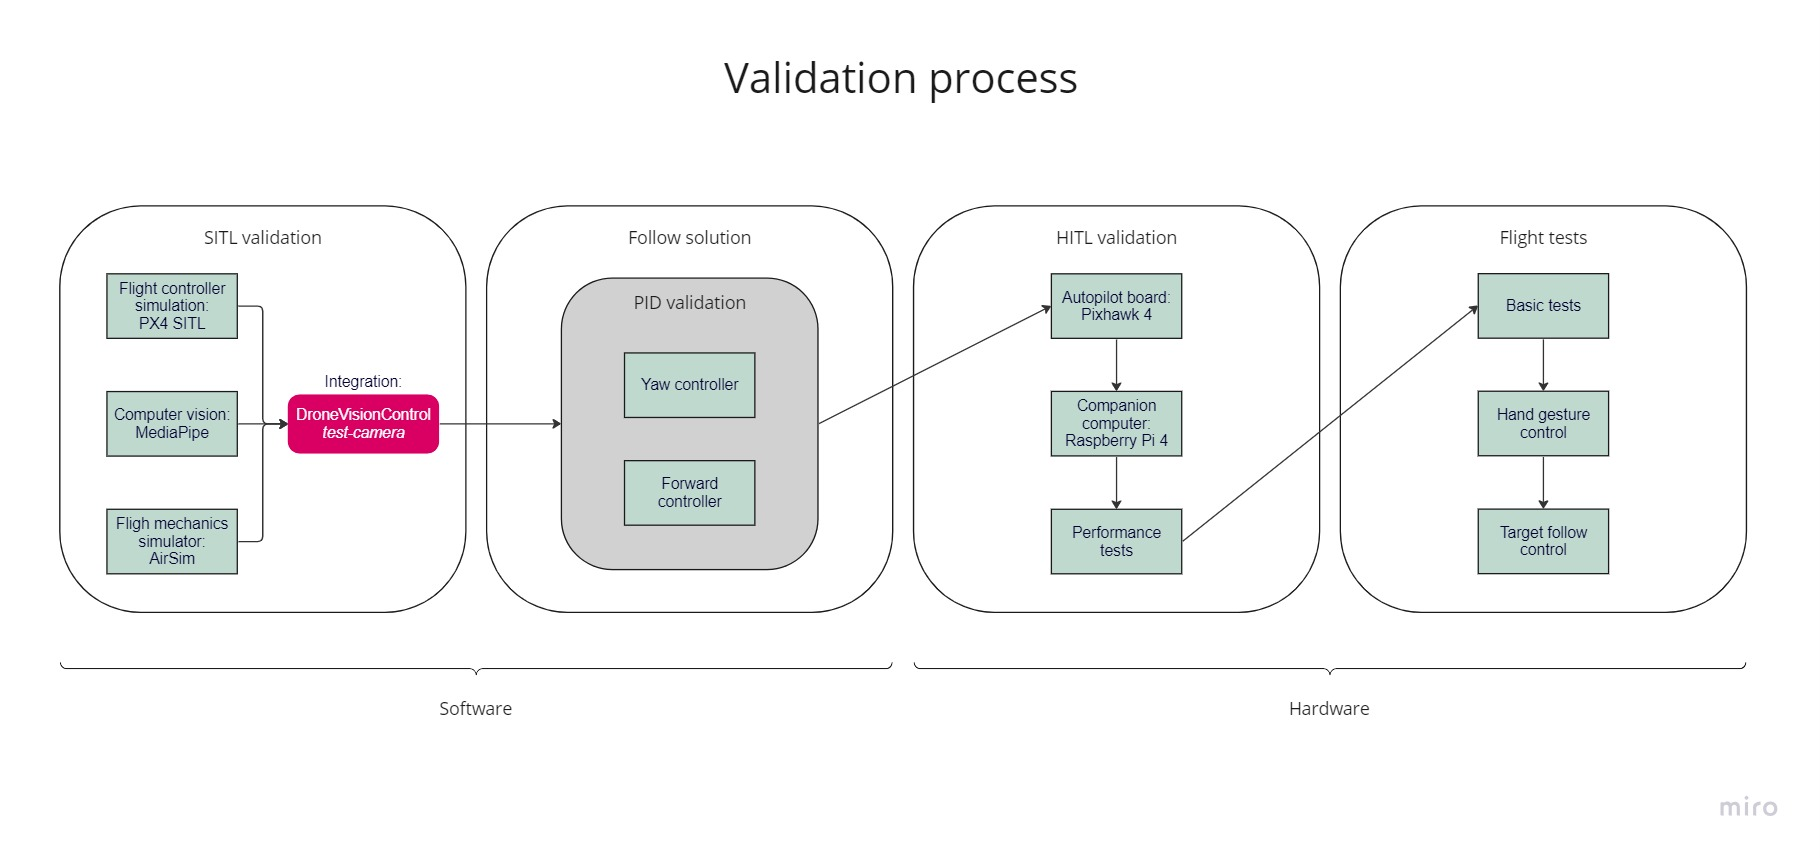
\includegraphics[width=\textwidth, keepaspectratio]{img/validation-chart.jpg}
  \caption{Outline for the validation process}\label{fig:validation-chart}
\end{figure}

\section{PX4 SITL simulation and validation}
\label{sec:test-2-sitl}

Section \ref{sec:devenv} describes the software-in-the-loop simulation mode developed by PX4.
By using this mode, it is possible to test and validate the correct operation of each individual part in the program's architecture.
To begin with, it is necessary to validate that it is possible to use the connection between the simulated flight controller and the dronecontrol program to send commands to the simulated vehicle, as well as being able to capture images from a connected camera and use them to test the detection algorithm.
The full list of validation steps is therefore:
\begin{enumerate}
    \item Verify that it is possible to start the simulated flight controller and that it connects to the 3D simulator vehicle.
    \item Connect the dronecontrol program to the flight controller and send basic commands.
    \item Retrieve images from a camera and run computer vision detection on them.
    \item Integrate the last three steps by running the hand-gesture control solution described in section \ref{sec:hands}
\end{enumerate}

For this purpose and to be able to run with a minimal configuration, the Gazebo simulator \footnote{\url{https://gazebosim.org/home}} included with the base PX4 installation will be used as the 3D environment.
This simulator works inside Linux in the same computer that runs the SITL PX4.
To be able to later transition into using the AirSim simulator instead, which runs in Windows, with minimal changes, for this test PX4, Gazebo and the dronecontrol program will run inside the Windows Subsystem for Linux.
The complete installation process necessary to run these tests is explained in appendix \ref{app:install-px4} and \ref{app:install-dronecontrol}.

\begin{figure}
  \centering
  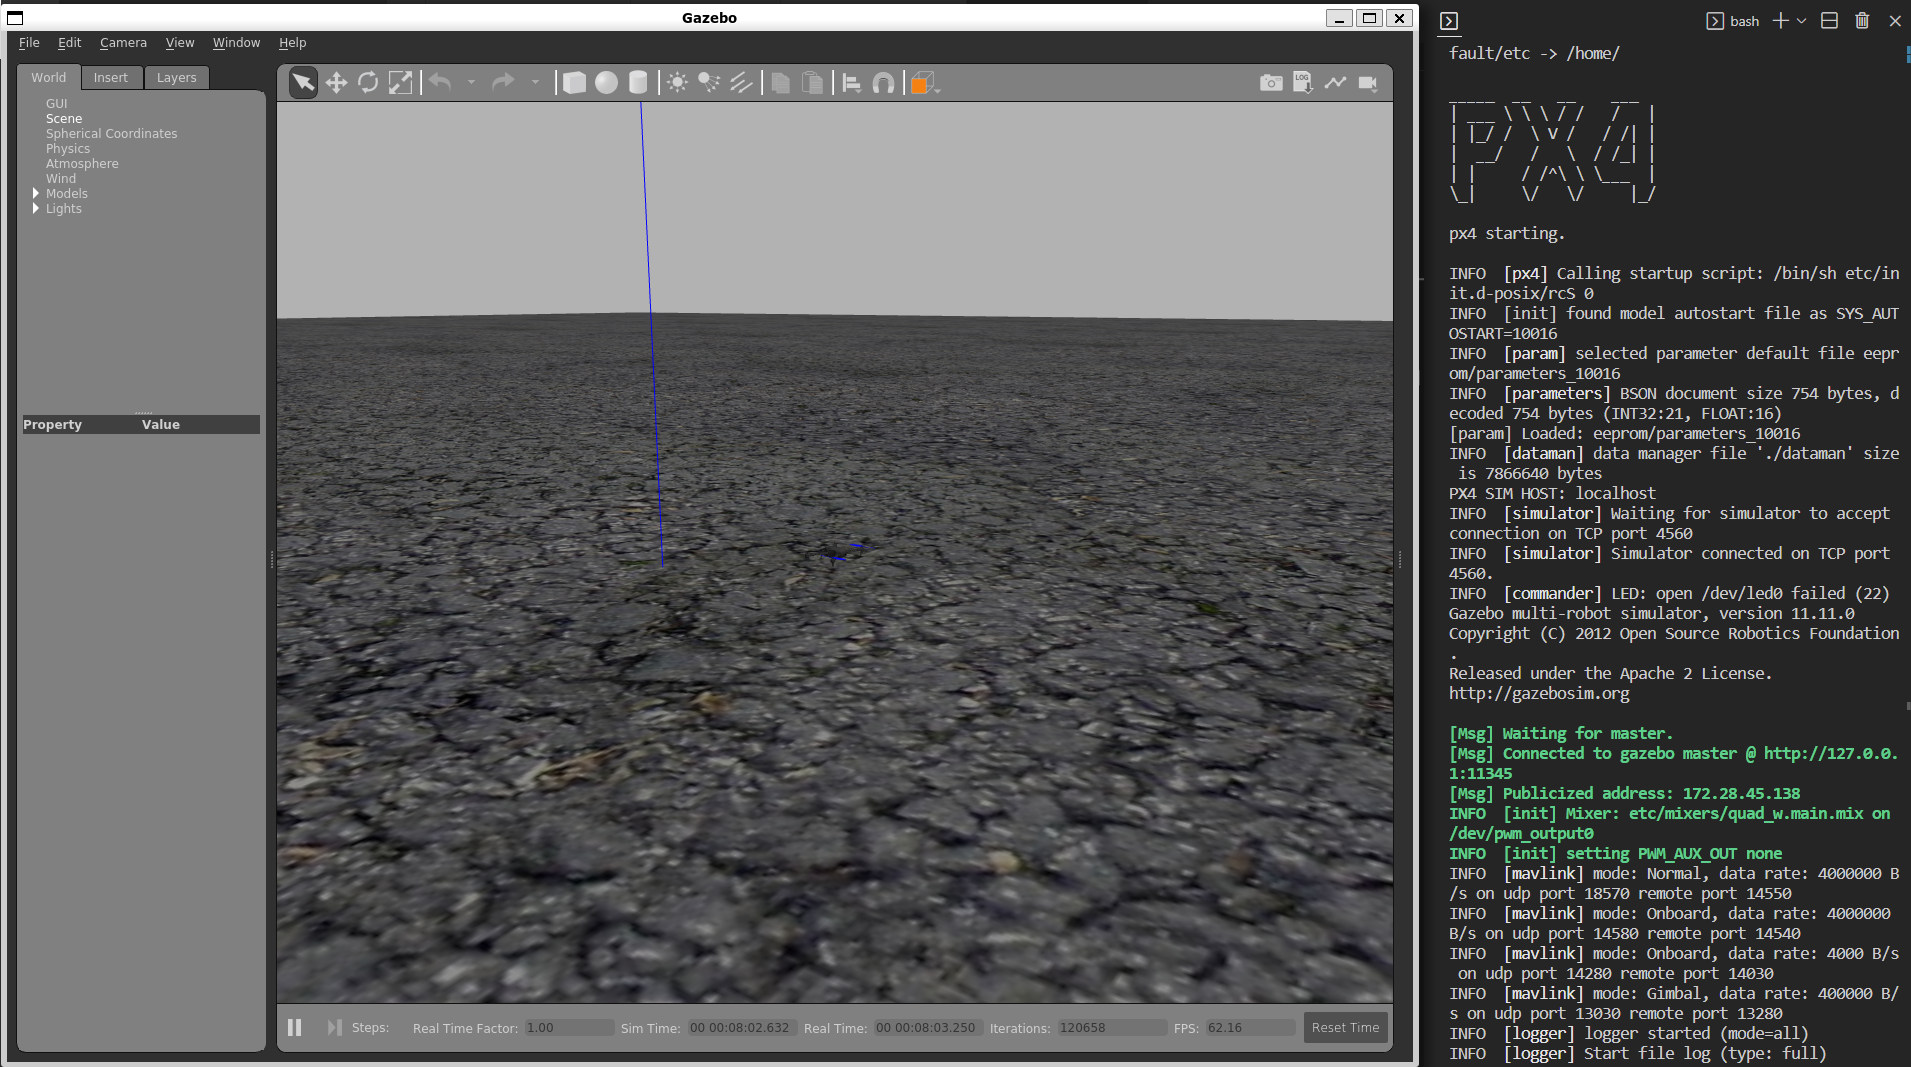
\includegraphics[width=.8\textwidth, keepaspectratio]{img/gazebo.png}
  \caption{Gazebo simulator (left) and output from the PX4 terminal (right) after PX4's software-in-the-loop mode is started}\label{fig:gazebo}
\end{figure}

Once both parts are installed, PX4 and Gazebo can be started by running the \mintinline{bash}{make px4_sitl gazebo} command inside its installation folder.
The result of this command can be seen in figure \ref{fig:gazebo}, where the left part shows the user interface and 3D world of the Gazebo simulator and the right side contains the PX4 console that can be used for sending commands and changing the configuration parameters of the simulated flight controller.
The simplest command to test is takeoff, which is done by sending \texttt{commander takeoff} through the console.
Figure \ref{fig:gazebo-takeoff} shows the state of the simulator after the takeoff command, with the vehicle model having climbed to the default height of 2.5 meters above ground.
To land the vehicle again, the command is \texttt{commander land}.

\begin{figure}
  \centering
  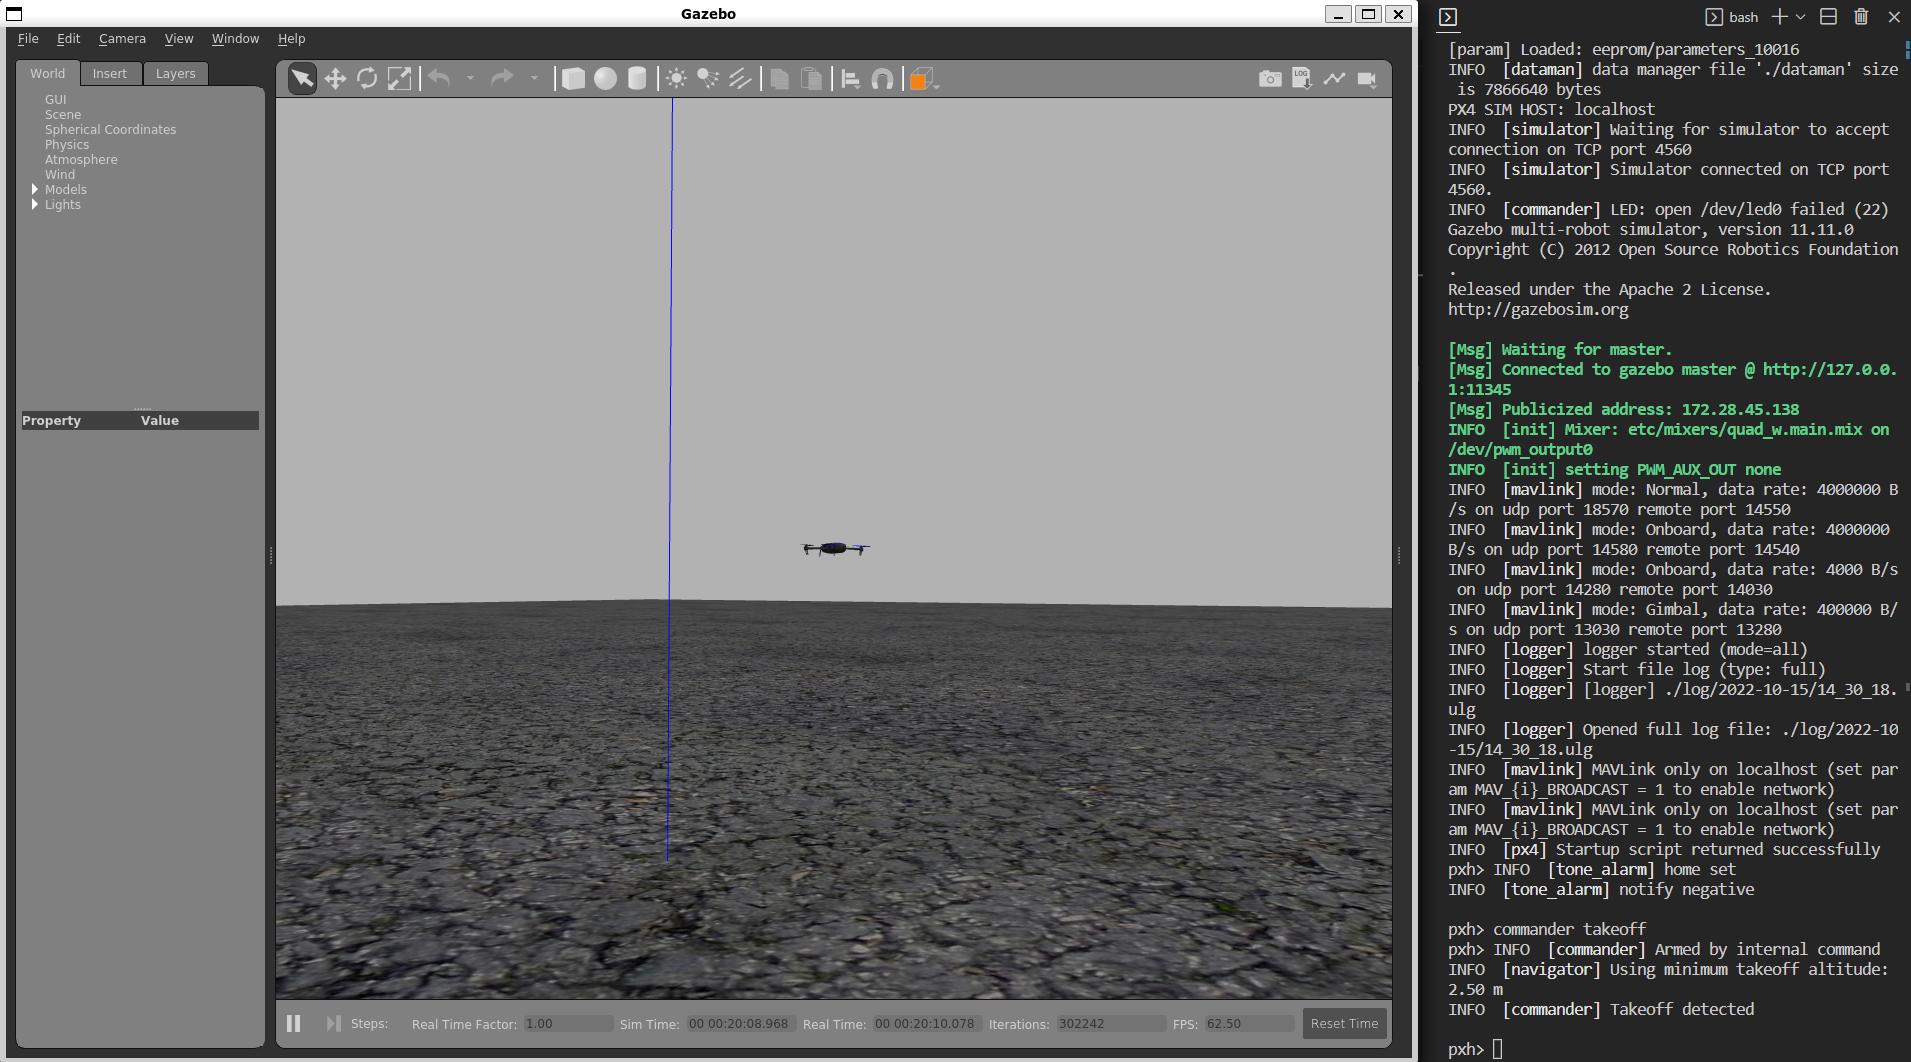
\includegraphics[width=.8\textwidth, keepaspectratio]{img/gazebo-takeoff.png}
  \caption{Gazebo simulator (left) and output from the PX4 terminal (right) after the takeoff command has been executed}\label{fig:gazebo-takeoff}
\end{figure}

The next step is to connect the dronecontrol application.
The camera testing tool described in section \ref{subsec:cam-tool} has been developed for this test, so that it is possible to establish a connection to PX4 SITL and process images without engaging any of the program's control modules.
The commands are then sent to PX4 through keyboard input, for example, the key "T" can be used to make the simulated vehicle take off.
Figure \ref{fig:sitl-hand} shows the image and text output of the program when the test camera tool is run with the hand detection feature activated.
On the left side, the detection algorithm tracks the joint of the hand present in the captured image and on the right side the logged information shows when the connection is established and keyboard commands are sent to the simulator.

\todo[inline]{Figure \ref{fig:sitl-hand}: Get a better image for this}
\begin{figure}
  \centering
  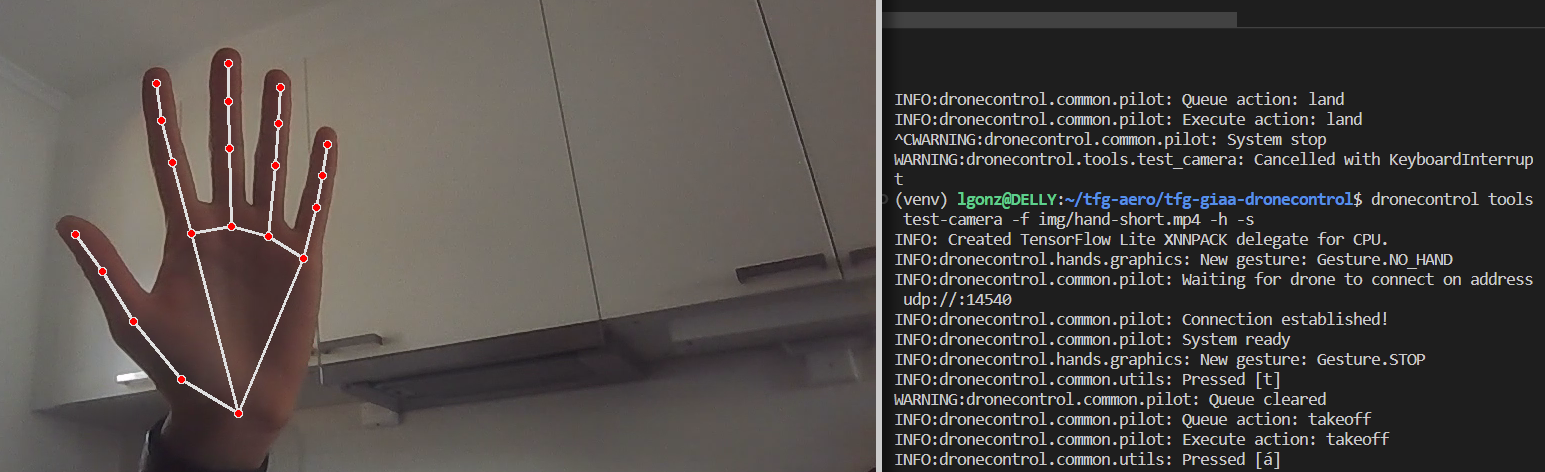
\includegraphics[width=\textwidth, keepaspectratio]{img/sitl-hand-2.png}
  \caption{Hand detection algorithm running on images taken from the computer integrated webcam}\label{fig:sitl-hand}
\end{figure}

The full execution of a test of the hand-gesture based control solution is shown in video in this link and excerpt of it can be seen in figure \ref{fig:sitl-hand-video}.
\todo[inline]{Video: Record video of hand-gesture solution running on SITL (+ screenshot on figure \ref{fig:sitl-hand-video})}

\begin{figure}
  \centering
  
\includegraphics[width=.6\textwidth, keepaspectratio]{img/placeholder.png}
  \caption{Single frame from the video showing the full execution of the hand-gesture control solution}
  \label{fig:sitl-hand-video}
\end{figure}


\subsection{PX4 SITL validation with AirSim}
\label{sec:test-3-airsim}

The end goal for the testing environment is for it to use the AirSim simulator to be able to take advantage of its 3D-world and computer vision capabilities.
For this reason, it becomes necessary to validate that the new simulator can run correctly on Unreal Engine on the computer and interact with PX4 as well as it did with the default Gazebo simulator and that all the necessary features for detection, tracking and following work as expected.
All these characteristics will be checked in the order below:
\begin{enumerate}
    \item Verify that the AirSim simulator is able to start, connect to the PX4 SITL through the WSL virtual network and receive commands from the PX4 terminal.
    \item Check that the dronecontrol program can connect to both AirSim through the WSL network to receive images and PX4 through the local network to send movement commands.
    \item Test the pose recognition algorithms on the images obtained from the AirSim simulation.
    \item Check that the follow solution is able to control the velocity of the vehicle directly in PX4's offboard mode.
\end{enumerate}

In the first place, the AirSim simulator needs to be installed in the Windows host.
The full installation process is described in appendix \ref{app:install-airsim}.
There are specific configuration parameters that have to be set to be able to connect the AirSim simulator in Windows to the PX4 SITL running inside WSL.
On the simulator side, AirSim's settings file has to include a line defining the IP address of the network interface to use.
This parameter, along with the full configuration file used for SITL testing can be found on appendix \ref{app:airsim-config}.
On the PX4 side, it is necessary to specify that the simulator will attach through a different IP address than \texttt{localhost}.
This is done by setting the \texttt{PX4\_SIM\_HOST\_ADDR} environment variable in the Linux system to the IP address of the Windows host on the WSL virtual network before starting PX4 as follows:
\begin{minted}{bash}
export PX4_SIM_HOST_ADDR=[IP-address]
make px4_sitl none_iris
\end{minted}
This starts the software-in-the-loop execution, which attempts to attach to an already running simulator listening on the IP address specified and the TCP port 4560, in this case, AirSim.
Therefore, every time one of PX4 or AirSim stops its execution, both of them have to be restarted in the specific order of first the AirSim simulator and then the PX4 flight controller.
Figure \ref{fig:airsim-sitl} shows the testing environment after the AirSim simulator and the PX4 console have been started successfully.

\todo[inline]{Figure \ref{fig:airsim-sitl}: Screenshot of PX4 console + Unreal with Airsim scene}
\begin{figure}
  \centering
  
\includegraphics[width=0.6\textwidth, keepaspectratio]{img/placeholder.png}
  \caption{AirSim environment connected to PX4 flight stack running in SITL mode}
  \label{fig:airsim-sitl}
\end{figure}

At this point, it is possible to use the PX4 console to send takeoff and land commands to the simulator and observe the 3D-model of the vehicle climb into the air.
To test the detection and tracking of human figures from images taken inside the simulator, one can again use the camera testing tool provided with dronecontrol.
Figure \ref{fig:airsim-sitl-pose} shows the output when the tool is run with the command \mintinline{bash}{dronecontrol tools test-camera --wsl --sim --pose-detection} and a 3D model of a person is situated in front of the drone in the simulated world.
In the image, the computer vision utilities detect the main features of the human body and a bounding box is drawn around it.
Meanwhile, the logged output from the program shows two calculated positions in the terminal: the x coordinate of the mid point of the bounding box and the percentage of the image height covered by the height of the bounding box.
These two numbers are the inputs for the PID controllers used in the follow solution as described in section \ref{sec:follow}, so that the output can be used to calibrate the distance from which the drone is to follow the person when that control mode is engaged.

\todo[inline]{Figure \ref{fig:airsim-sitl-pose}: dronecontrol console + Unreal with Airsim scene + image output running test-camera}
\begin{figure}
  \centering
  
\includegraphics[width=0.6\textwidth, keepaspectratio]{img/placeholder.png}
  \caption{AirSim, PX4 and dronecontrol applications running side-by-side and connecting to each other}
  \label{fig:airsim-sitl-pose}
\end{figure}

Now that the testing environment is working as expected and before it is used to tune the PID controllers in the follow solution to the response of the vehicle's movement in the next section, it is possible to verify that the controllers are capable of reacting to changes in the position of the figure by only enabling their proportional term with an appropriately low magnitude to keep the movement slow and smooth.
The drone movement when running the follow control program with values of 10 and 2 on the proportional term of the yaw and forward controllers, respectively, which can be done with the command \mintinline{bash}{dronecontrol follow --sim --yaw-pid (10, 0, 0) --fwd-pid (2, 0, 0)}, is shown in video format in this link and a frame extracted from it can be seen in figure \ref{fig:airsim-test-follow}.


 \todo[inline]{Video: Record video of follow solution running on AirSim + SITL (+ screenshot for figure \ref{fig:airsim-test-follow})} 
\begin{figure}
  \centering
  
\includegraphics[width=.6\textwidth, keepaspectratio]{img/placeholder.png}
  \caption{Single frame from the video showing the movement of the drone in response to changes in position of the tracked person}
  \label{fig:airsim-test-follow}
\end{figure}
\clearpage

\section{PID controller validation}
\label{sec:test-1-pid}

% Process of tuning the PIDs
% Graphs from test-controller
% Analysis of error

As mentioned before, the velocity controller that is the heart of the person following mechanism is based on two PID controllers.
In order to get velocity outputs for the PID controllers that produce a stable movement of the vehicle, it is necessary to tune the parameters of the controllers until the appropriate combination is found.
In this section, the value for the coefficients used for the project will be found empirically with the help of the tuning tool described in section \ref{subsec:pid-tools} and developed for this purpose. Its performance will be validated with the controller testing tool, both running in the simulated environment with the flight stack in SITL mode so that it is possible to take continuous measures of the response of the PID controllers to step movements of a simulated person present in the 3D world.
In the first place, each controller will be tuned independently of the other by allowing the vehicle only one direction of movement at a time.
Afterwards, both controllers are engaged simultaneously to measure the joint response to a range of different inputs.

The controllers are calibrated for a reference position of x=0, y=0 for the vehicle and x=600, y=0 for the person in world coordinates of the simulated environment.
At these positions, processed images taken from the simulated camera detect the person centred in the field of view and with a height of 36\% of the image height.
This means that the controllers running in the simulator will have as their target set points 0.5 for the yaw controller and 0.36 for the forward controller. 
So for any changes in the position of the simulated person, the controllers will send velocity commands to the autopilot to achieve the same relative position between the vehicle and the person as in the reference shown in figure \ref{fig:tune-start-pos}.

\begin{figure}
  \centering
  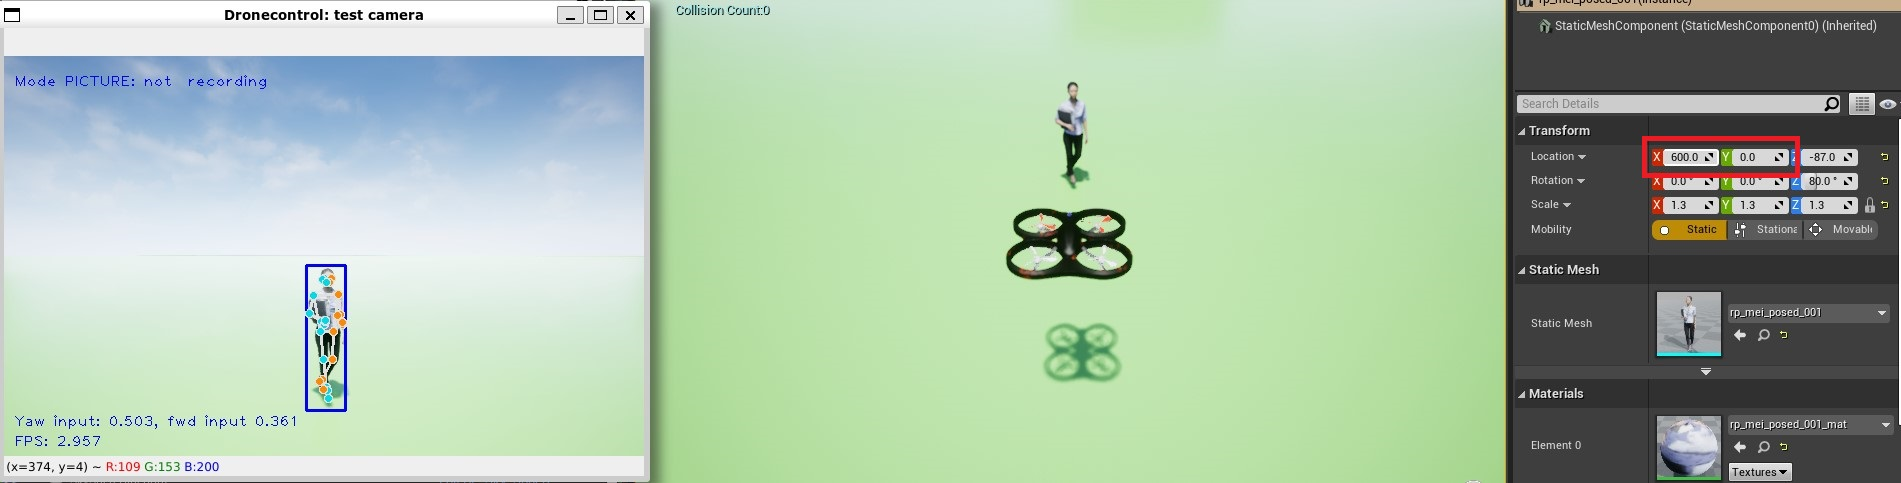
\includegraphics[width=\textwidth, keepaspectratio]{img/pid/tune-ref-pos.jpg}
  \caption{Reference position for the yaw and forward PID controllers. From left to right, the panels show the dronecontrol application window, the AirSim simulator world view and the world location of the human model in the simulator. The distance between the vehicle and the person is 600 units in the x direction and 0 units in the y direction.}
  \label{fig:tune-start-pos}
\end{figure}


\subsection{Yaw controller}

\begin{figure}
  \centering
  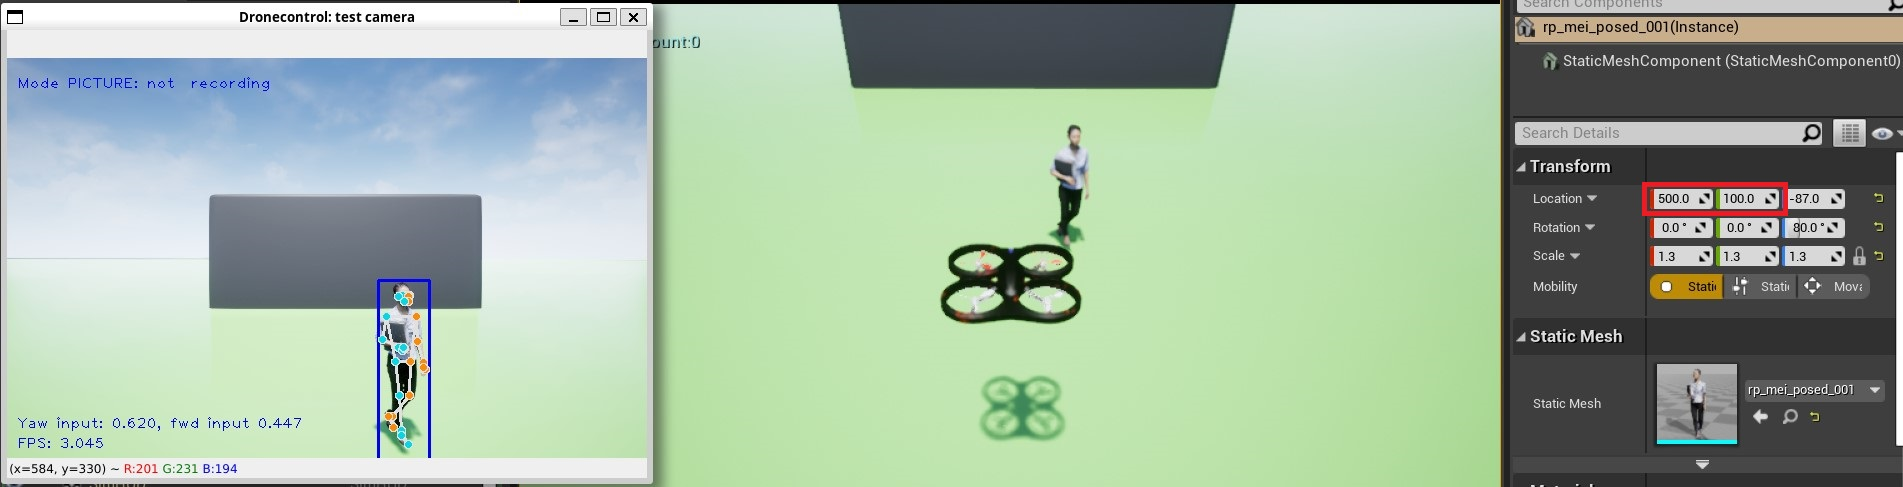
\includegraphics[width=\textwidth, keepaspectratio]{img/pid/tune-ref-pos-yaw.jpg}
  \caption{Starting position of the simulator for tuning the yaw controller. The human model is situated 500 units forward and 100 units to the right of the vehicle model.}
  \label{fig:tune-ref-pos-yaw}
\end{figure}

To find the correct coefficients for the controller that governs the yaw velocity of the vehicle, the target person is set in a position slightly to the side on its field of view so that when the controller is engaged, it outputs a rotation of the vehicle to that side.
Since the forward controller will not be engaged during the test, the target person can be situated closer to the camera to make it easier for the pose detection algorithm to output correct landmarks.
Figure \ref{fig:tune-ref-pos-yaw} shows the starting position of the simulated environment before each run, where the 3D model has been situated at (500, 100), that is, 100 units to the right of the reference position.
On the left-most panel of figure \ref{fig:tune-ref-pos-yaw}, the dronecontrol application shows that the input to the yaw controller is 0.62 at this position.
The controller must then output a positive yaw velocity to centre the person in its field of view. 
This offset position to the right produces an error that is less than zero (set point minus input, $\epsilon = 0.5 - 0.62$ ).
However, it requires a positive velocity to counteract and induce a yaw velocity to the right, so the coefficients for the yaw controller will need to be negative so that an increased horizontal position results in a positive yaw velocity to decrease it, as indicated by equation \ref{eq:pid}.
 

\begin{figure}
  \centering
  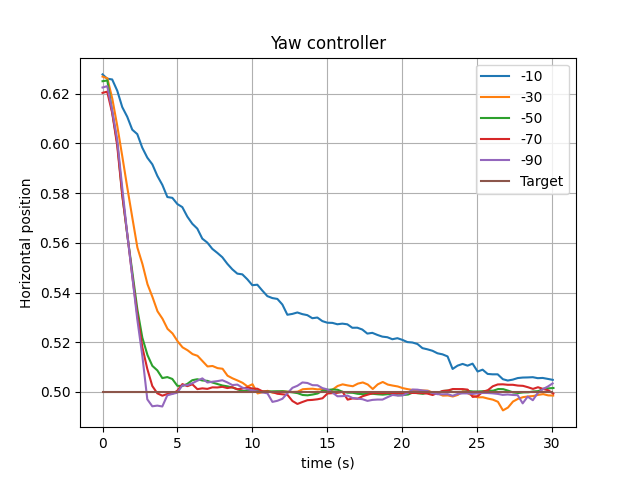
\includegraphics[width=.45\linewidth]{img/pid/yaw/yaw_pos_prop_i0_d0.png}
  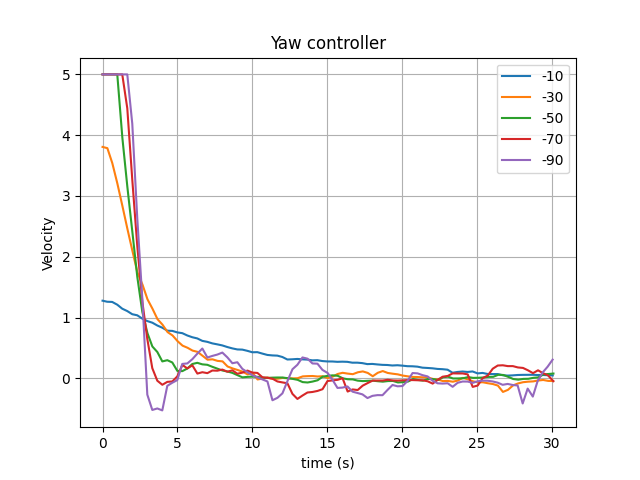
\includegraphics[width=.45\linewidth]{img/pid/yaw/yaw_vel_prop_i0_d0.png}
  \caption{Variation of (a) input position and (b) output velocity for different values of $K_{P}$ and $K_I=0$, $K_D=0$ while the yaw controller is engaged.}\label{fig:tune-yaw-prop}
\end{figure}

To tune the controller to its correct coefficients, the first step will be to test different values of $K_{P}$ while maintaining $K_{I}$ and $K_{D}$ at zero.
Figure \ref{fig:tune-yaw-prop} shows the output of the tuning program for the five values of $K_{P}$ tested, from $K_P=-10$ to $K_P=-90$ in increments of 20.
The left graph represents the variation of the horizontal position detected by the camera for the first 30 seconds after activating the controller.
The right graph shows the yaw velocity that the controller outputs to the pilot module to reach the target.
For low values of $K_{P}$, the controller makes the vehicle move slowly towards its target so that it takes a long time to reach the midpoint position.
On the other hand, for high values of $K_{P}$, the controller tries to reach the target too fast, so when it gets close to it, it starts to oscillate around the target.
The right side graph also shows well how the output velocity in the yaw controller is limited to 5 degrees per second, so even for very high values of $K_P$, the vehicle will not rotate faster than that.
From the graphs, the best of the values tested is $K_{P}=50$, where the distance to the target point decreases rapidly (left graph), but the velocity does not start to increase and decrease widely around 0 (right graph).

The second step is to find the correct value for $K_I$. 
To do that, several values of $K_I$ will be tested for a low $K_P$ of -20 and $K_D=0$ so that the effect of the integral part is easier to appreciate. Figure \ref{fig:tune-yaw-int-20} shows the evolution of the input and output at the controller for a sample time of 40 seconds for each of the values tested. 
For a low $K_I=-1$, the progress toward the target is stable and slightly faster than without any contribution of the integral part.
However, when the $K_I$ increases in magnitude, it creates initial oscillations around the target position that fade out as time progresses. For a very large $K_I$ from around -10, the vehicle's velocity becomes locally unstable with many slight variations in its oscillations.

\begin{figure}
  \centering
  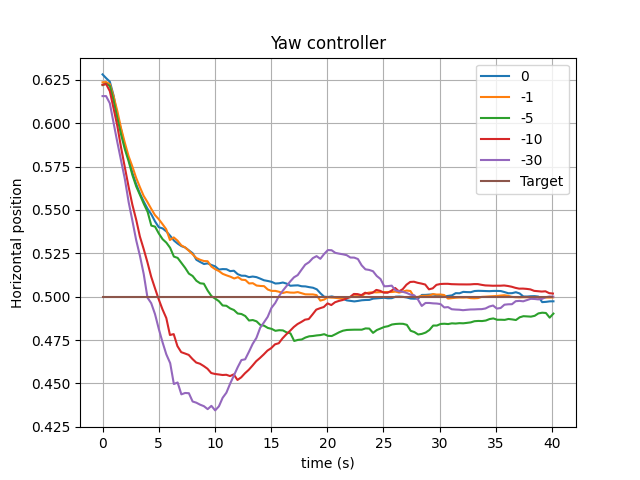
\includegraphics[width=.45\linewidth]{img/pid/yaw/yaw_pos_p20_int_d0.png}
  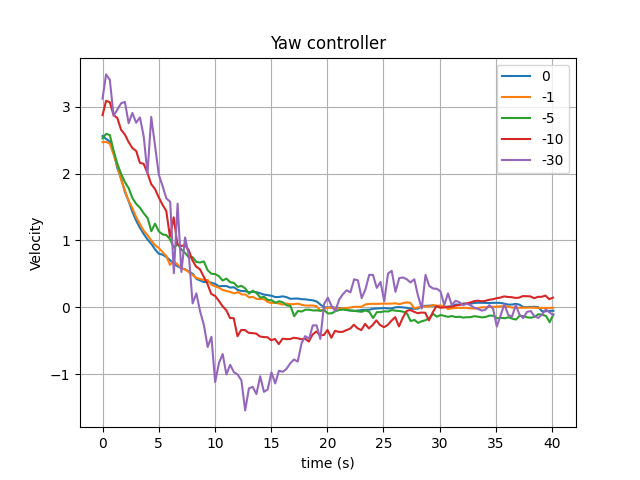
\includegraphics[width=.45\linewidth]{img/pid/yaw/yaw_vel_p20_int_d0.png}
  \caption{Variation of (a) input position and (b) output velocity for different values of $K_{I}$ and $K_P=-20$, $K_D=0$ while the yaw controller is engaged.}\label{fig:tune-yaw-int-20}
\end{figure}

A similar effect can be observed to a lower extent in figure \ref{fig:tune-yaw-int-50}, where the measurements have been taken for $K_P=-50$ and $K_D=0$. 
In this graph, $K_I=-1$ makes the controller reach the target position some 3 seconds faster and with similar oscillations in its velocity than with the proportional part exclusively ($K_P=-50$, $K_I=0$, $K_D=0$).

\begin{figure}
  \centering
  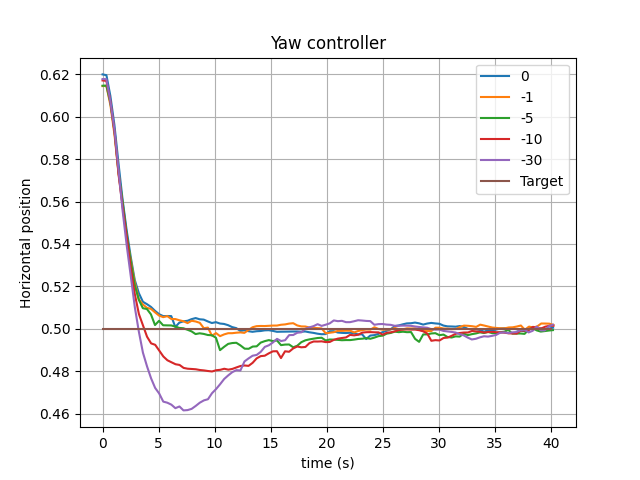
\includegraphics[width=.45\linewidth]{img/pid/yaw/yaw_pos_p50_int_d0.png}
  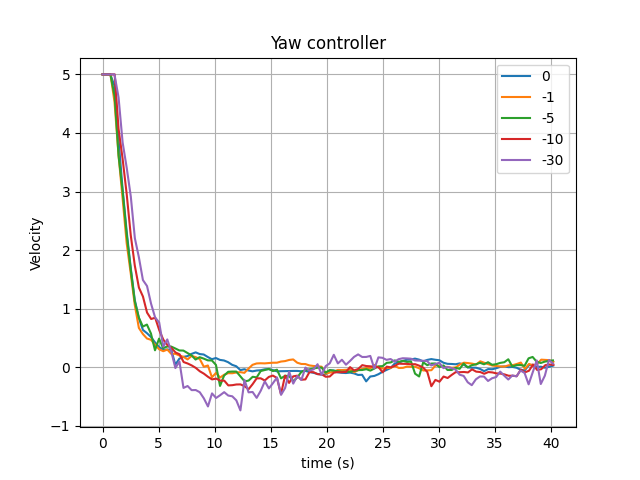
\includegraphics[width=.45\linewidth]{img/pid/yaw/yaw_vel_p50_int_d0.png}
  \caption{Variation of (a) input position and (b) output velocity for different values of $K_{I}$ and $K_P=-50$, $K_D=0$ while the yaw controller is engaged.}\label{fig:tune-yaw-int-50}
\end{figure}

In the last step, the tuning process will deal with the derivative part of the controller.
In this case, several values of $K_D$ have been tested against the chosen $K_P=-50$, both without any integral part and with $K_I=-1$.
This will allow seeing the effect that the derivative part has in the controller, as well as validating if the integral part chosen in the last step can work together with the derivative part to make the controller react better to a changed input.
Figures \ref{fig:tune-yaw-der-i0} and \ref{fig:tune-yaw-der-i1} show the evolution of the position detected by the computer vision system and the velocity the controller outputs for a sample time of 40 seconds for $K_I=0$ and $K_I=-1$, respectively, with $K_P=-50$.
For all the tested values, the iteration with $K_I=-1$ on \ref{fig:tune-yaw-der-i1} shows a better convergence towards the target positions than their counterpart values of $K_D$ for $K_I=0$, which indicates that the integral part has been chosen correctly.
Furthermore, adding any amount to the derivative part does not produce any visible benefit in the step response of the controller and the curve that first stabilises on the target position continues to be the one for $K_D=0$, while the velocity graph remains approximately the same between $K_D=0$ and $K_D=-2$
The final values for the coefficients for the yaw controller will then be $K_P=-50$, $K_I=-1$, and $K_D=0$, so the controller will, in truth, only be a PI controller and not a complete PID controller.


\begin{figure}
  \centering
  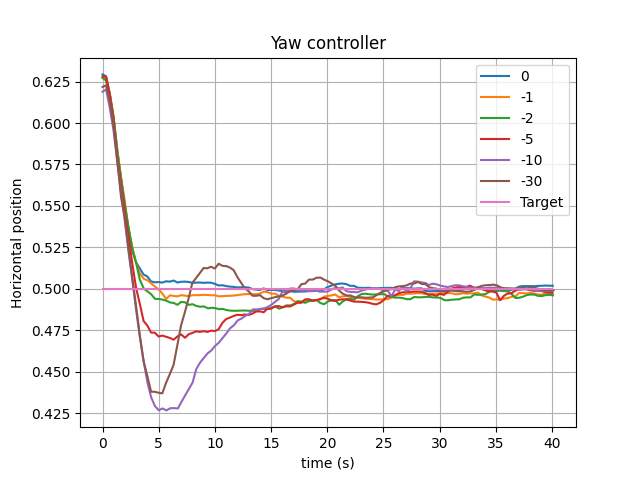
\includegraphics[width=.45\linewidth]{img/pid/yaw/yaw_pos_p50_i0_der.png}
  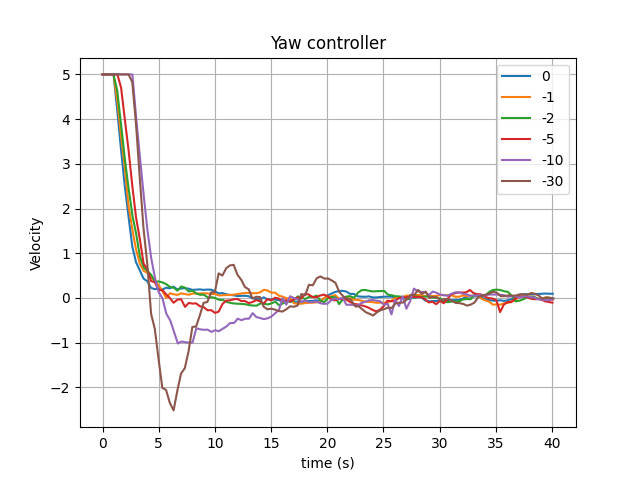
\includegraphics[width=.45\linewidth]{img/pid/yaw/yaw_vel_p50_i0_der.png}
  \caption{Variation of (a) input position and (b) output velocity for different values of $K_{D}$ and $K_P=-50$, $K_I=0$ while the yaw controller is engaged.}\label{fig:tune-yaw-der-i0}
\end{figure}

\begin{figure}
  \centering
  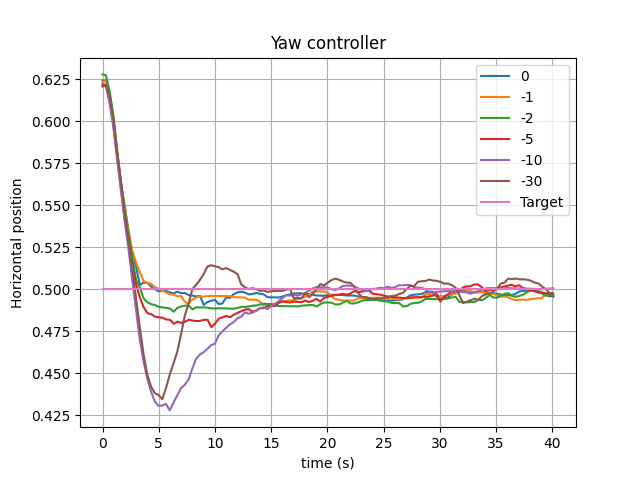
\includegraphics[width=.45\linewidth]{img/pid/yaw/yaw_pos_p50_i1_der.png}
  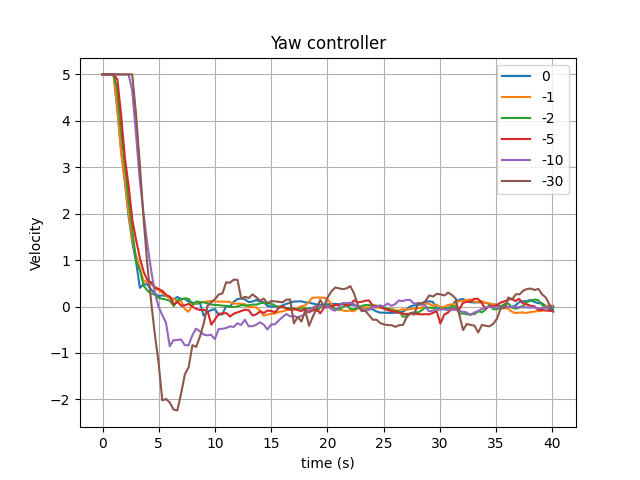
\includegraphics[width=.45\linewidth]{img/pid/yaw/yaw_vel_p50_i1_der.png}
  \caption{Variation of (a) input position and (b) output velocity for different values of $K_{D}$ and $K_P=-50$, $K_I=-1$ while the yaw controller is engaged.}\label{fig:tune-yaw-der-i1}
\end{figure}

A recording of the whole tuning process for the yaw controller can be seen in this \href{https://l-gonz.github.io/tfg-giaa-dronecontrol/videos/tune-yaw-controller}{video}\footnote{\url{https://l-gonz.github.io/tfg-giaa-dronecontrol/videos/tune-yaw-controller}}.


\subsection{Forward controller}


A similar process to the one used for the yaw controller must be followed for the forward controller.
The starting position for the tuning process is, in this case, with the figure closer to the vehicle than the reference position and centred in its field of view.
Figure \ref{fig:tune-ref-pos-fwd} shows this starting setup with the figure situated at the (450,0) position in the simulated world.
In this position, the input to the forward controller is 0.47, that is, the bounding box around the detected figure takes up 47\% of the height of the camera field of view.
The response from the controller will therefore need to be a negative forward velocity that brings the vehicle away from the target person to reduce the perceived figure height.
Since a negative output velocity reduces the input at the entrance of the controller in a directly proportional manner, the coefficients for this PID controller will need to be positive, contrary to what happened on the yaw controller where the feedback loop was inversely proportional (a positive velocity decreased the input to the yaw controller).


\begin{figure}
  \centering
  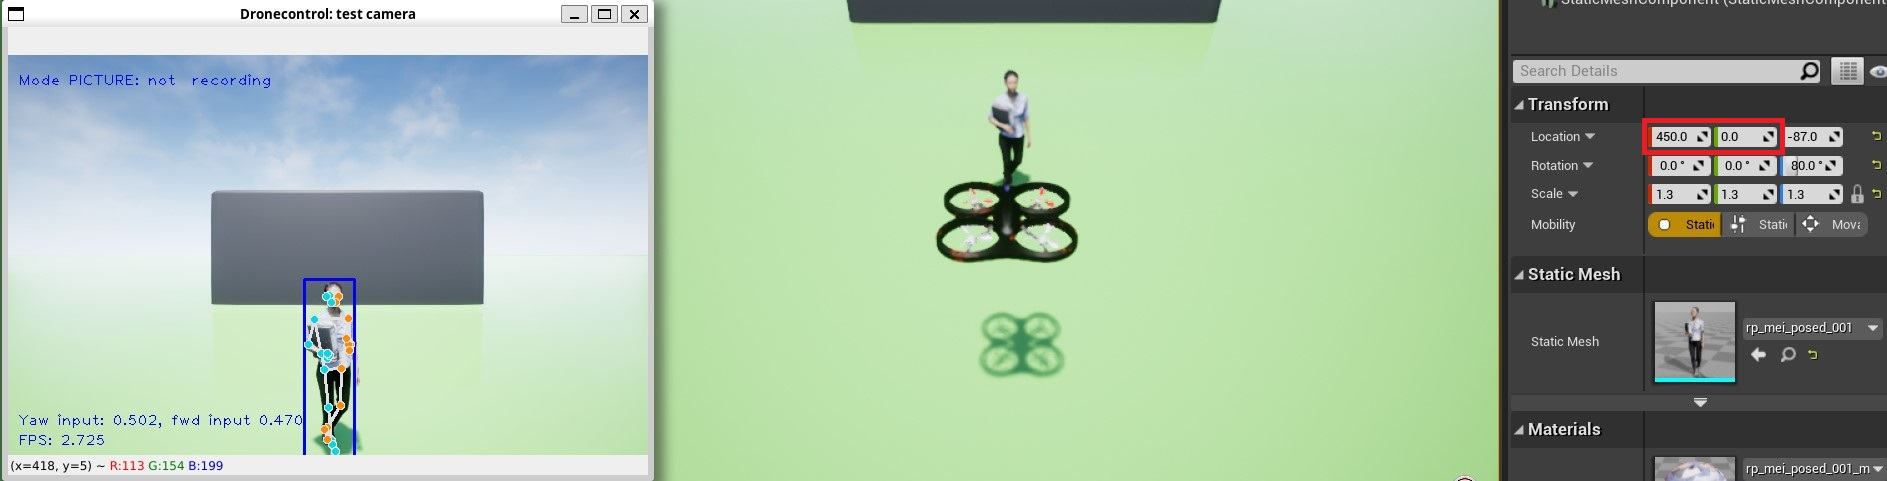
\includegraphics[width=\textwidth, keepaspectratio]{img/pid/tune-ref-pos-fwd.jpg}
  \caption{Starting position of the simulator for tuning the forward controller. The human model is situated 450 units forward and centred from the vehicle position.}\label{fig:tune-ref-pos-fwd}
\end{figure}

In general, the forward velocity will always need to be smaller than the yaw velocity since it induces a pitch angle in the vehicle that tilts the camera up and down, which can destabilise the camera and cause a loss of sight of the followed figure.
To achieve that, the coefficients for the forward controller will be reduced by one order of magnitude.
First, values from $K_P=1$ to $K_P=9$ in increments of 2 have been tested for $K_I=0$ and $K_D=0$ for a sample time of 30 seconds.
The curves described by the controller for these coefficients are shown in figure \ref{fig:tune-fwd-prop}.
Compared with the trajectory described by the yaw controller, the forward controller is generally more unstable since fast forward and backwards movements affect the pose detection algorithm.
This is particularly visible at the start of each test as slightly different heights are detected in the image from the camera even though the vehicle is in the same position with respect to the human figure.
It also creates an effect, especially for the bigger $K_P$ values tested, where, as the vehicle begins its movement back to its target position, the pose detection mechanism gets a slightly different perspective on the followed person, which increases the detected height slightly so that small spikes of detected differences show in the height graphs even though the velocity graph shows that the vehicle's direction of movement remains the same.
This effect is reduced by keeping the output forward velocity small in the controller.
In the right graph of figure \ref{fig:tune-fwd-prop}, it is also visible for high values of $K_P$ how the output velocity increases enough that the maximum velocity limit is reached on the forward controller and the output is capped to \unitfrac[0.4]{m}{s}.
For a value up to $K_P=3$, the trajectory described descends rapidly without ending in significant oscillations around the target height, so it is a fair value to keep for the final controller.


\begin{figure}
  \centering
  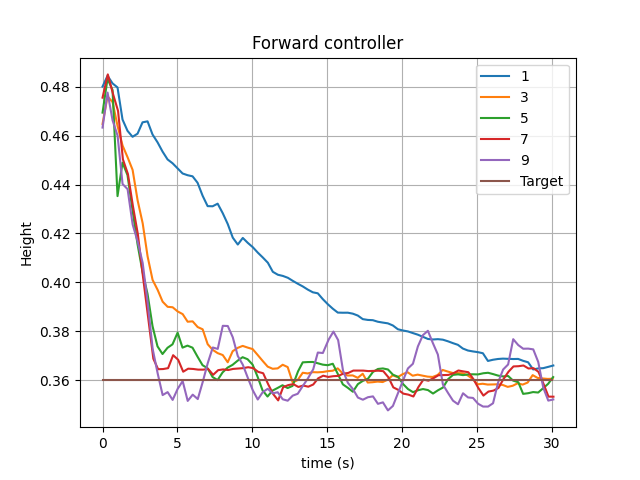
\includegraphics[width=.45\linewidth]{img/pid/fwd/aaa_fwd_pos_prop_i0_d0.png}
  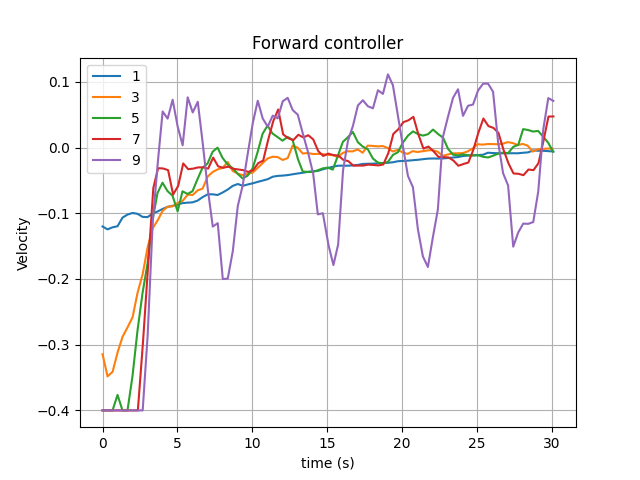
\includegraphics[width=.45\linewidth]{img/pid/fwd/aaa_fwd_vel_prop_i0_d0.png}
  \caption{Variation of (a) input height and (b) output velocity for different values of $K_{P}$ and $K_I=0$, $K_D=0$ while the forward controller is engaged.}\label{fig:tune-fwd-prop}
\end{figure}


The respective tests for $K_I$ and $K_D$ in the forward controller are shown in figures \ref{fig:tune-fwd-int} and \ref{fig:tune-fwd-der}.
Increasing the coefficient for the integral part causes the controller to overshoot the target initially but then stabilise before starting to approximate to the target position.
Since, for this application, overshooting is not desirable, as it can cause safety issues, the chosen value of $K_I$ will be 0.
For the derivative part, every value of $K_D$ tested increases the system's oscillations, so it will also be left out of the forward controller.
The final values for the coefficients for the forward controller will then be $K_P=3$, $K_I=0$, and $K_D=0$, which makes it only a proportional controller.


\begin{figure}
  \centering
  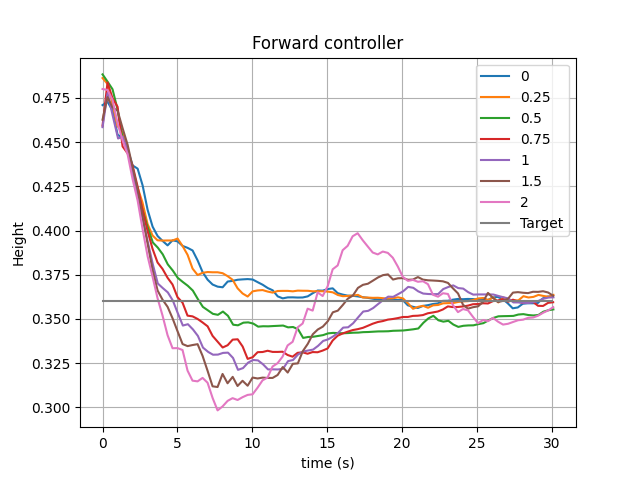
\includegraphics[width=.45\linewidth]{img/pid/fwd/aaa_fwd_pos_p3_int_d0.png}
  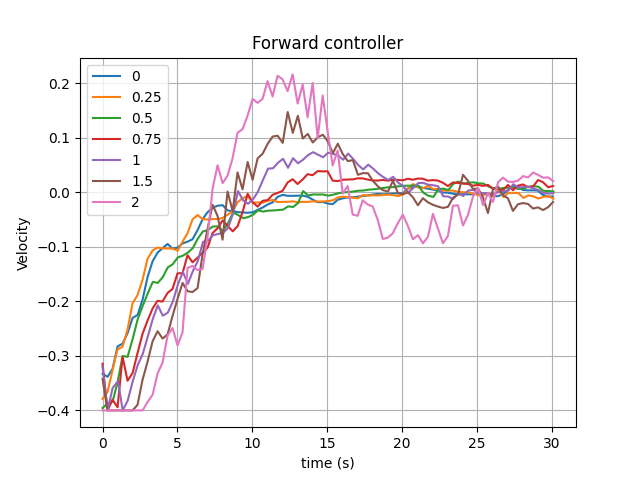
\includegraphics[width=.45\linewidth]{img/pid/fwd/aaa_fwd_vel_p3_int_d0.png}
  \caption{Variation of (a) input height and (b) output velocity for different values of $K_{I}$ and $K_P=7$, $K_D=0$ while the forward controller is engaged.}\label{fig:tune-fwd-int}
\end{figure}
\begin{figure}
  \centering
  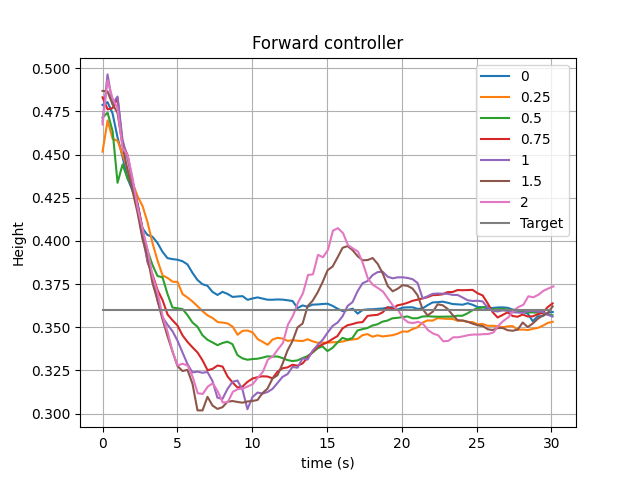
\includegraphics[width=.45\linewidth]{img/pid/fwd/aaa_fwd_pos_p3_i0_der.png}
  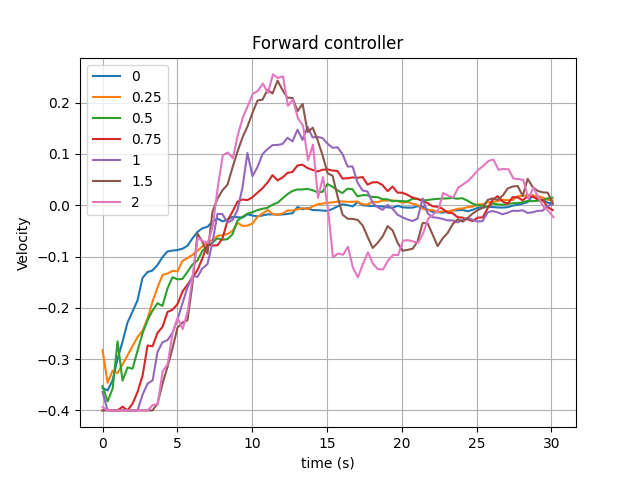
\includegraphics[width=.45\linewidth]{img/pid/fwd/aaa_fwd_vel_p3_i0_der.png}
  \caption{Variation of (a) input height and (b) output velocity for different values of $K_{D}$ and $K_P=7$, $K_I=0.5$ while the forward controller is engaged.}\label{fig:tune-fwd-der}
\end{figure}


\subsection{PID tuning validation}
\label{subsec:pid-test-controller}

As a final validation for the tuning obtained previously, the \texttt{test-controller} tool described in section \ref{subsec:pid-tools} will be used to check the step response of the controllers to different starting distances for the same coefficients.
Additionally, for this test, both controllers will be engaged simultaneously to verify that they work well together.
Firstly, the positions will vary on the y-axis, that is, the figure will move from left to right in the field of view of the vehicle.
The values for the y coordinate to be tested will be between -150 and 150 units in increments of 50.
The x coordinate of the figure in the simulated world will remain at $x=500$.

Plots of the changes in normalised horizontal distance and normalised figure height detected by the person recognition algorithm during the time the vehicle takes to reach the target distance from the human figure for each of the tested positions can be seen in figure \ref{fig:validate-yaw}.
It is considered that the vehicle has reached its target when the error is less than 2\%, and the output speed at the controller is less than 10\% of the maximum value.
Furthermore, the whole testing process followed with the developed \texttt{test-controller} tool can be seen in this \href{https://l-gonz.github.io/tfg-giaa-dronecontrol/videos/test-yaw-controller}{video}\footnote{\url{https://l-gonz.github.io/tfg-giaa-dronecontrol/videos/test-yaw-controller}}.

Since each starting position differs in distance and orientation to the target, both controllers must be engaged to reach the centre.
The yaw controller then introduces a negative yaw velocity when the figure is on the left half of the camera's field of view and a positive yaw velocity when the figure is on the right half to reach the target horizontal distance of 0.5 (figure centred in the image received from the camera);
Moreover, the forward controller outputs a negative forward velocity to reduce the detected height of the figure from around 0.44 to the target 0.36 since the figure is 100 units closer to the vehicle than the reference position $x=600$.

Figure \ref{fig:validate-yaw}a shows that the most time is spent on starting the movement towards the target and, after that, there is not much difference between the time it takes to reach the -50 position and reaching the -150 position, with the former taking 3 seconds and the later taking around 3.6 seconds.
In figure \ref{fig:validate-yaw}b, all of the trajectories have a very similar graph since the starting distance to the target is practically the same, where the controller makes the vehicle pull backwards so the figure stays far enough, making the detected height decrease.
For the $y=100$ starting position, the initial detected height is very small in the beginning until it reaches the starting point of the other tests.
This occurred because the detection algorithm took longer than usual to identify the person in this particular test.
However, after less than half a second, the detection was stabilised without affecting much the time it took to reach the target or its final position, showing that the controllers can recover from errors in the detection mechanism without affecting the vehicle's movement.


\begin{figure}
  \centering
  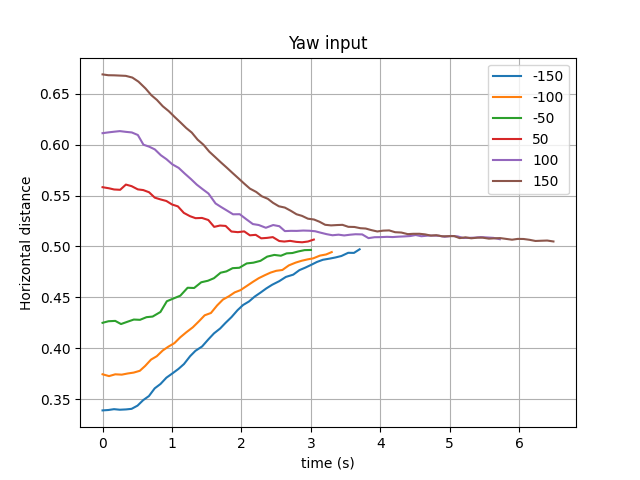
\includegraphics[width=.45\linewidth]{img/pid/validation_yaw.png}
  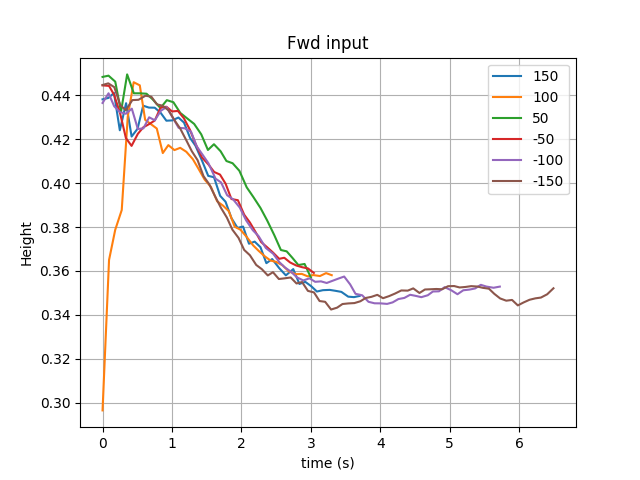
\includegraphics[width=.45\linewidth]{img/pid/validation_yaw_2.png}
  \caption{Changes over time in detected horizontal position and height as input for the controllers with different starting positions in the y-axis}
  \label{fig:validate-yaw}
\end{figure}

Additionally, the \texttt{test-controller} tool can be run with varying positions in the x-axis, which means that the tests are run with the human figure at different distances closer and further away from the vehicle while maintaining it in the centre of its field of view (y position will remain 0 for the whole process).
Therefore, the yaw controller will not need to be considered for this test.
The changes over time in the input into the forward controller between each starting position and the target position are shown in figure \ref{fig:validate-fwd}.
The figure reflects a significant difference in how the controller reacts to positions closer than the target distance or further from it.
When the person is very close to the vehicle, there are major differences between detected heights, so the vehicle moves fast away from its position.
However, when the person is further away from the vehicle than the target, large differences in distance are associated with minor differences in detected height, which causes the controller to determine a smaller velocity increase than for the same distance difference if the person was closer to the vehicle.
Therefore it will take a longer amount of time for the vehicle to reach the target.
It is worth noting that even when the person is so close to the vehicle that part of it falls outside of its field of view ($x=300$ in the figure), the pose detection works well enough to interpret where the person should continue outside of the image so that it is still possible for the controller to decide the correct direction of movement.

\begin{figure}
  \centering
  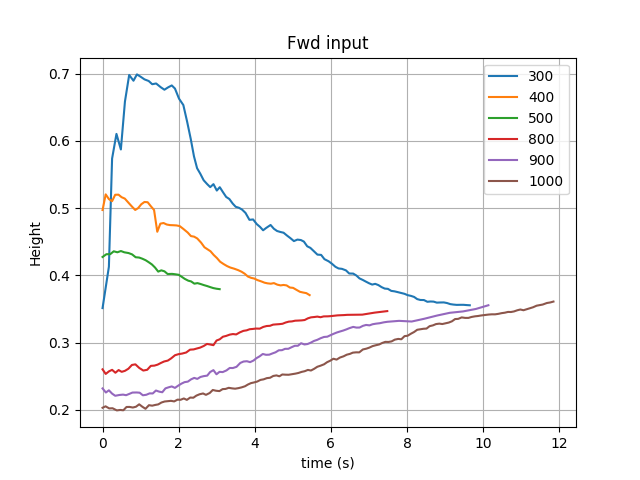
\includegraphics[width=.8\textwidth, keepaspectratio]{img/pid/validation_fwd.png}
  \caption{Changes over time in detected height as input for the forward controller with different starting positions in the x-axis}
  \label{fig:validate-fwd}
\end{figure}


\clearpage

\section{PX4 HITL simulation and validation}
\label{sec:test-4-hitl}

% Setup:    build drone, HITL configuration
% Test:     - AirSim + follow on Windows + Pixhawk
%           - QGroundControl (without program running)
%           - PX4 to computer connection
%           - RC on AirSim
% Results:  images of wiring computer-Pixhawk

The aim of this section is to validate the transition from using a simulated version of the flight stack running on Linux (PX4's software-in-the-loop simulation) to using a physical Pixhawk board with simulated input and output to test the flight controller interaction with the developed program.
To do so, the aim is to be able to run the follow solution to send control commands through the Pixhawk board and observe the movement of the vehicle in the AirSim simulator in the same manner as in the previous section.


QGroundControl contains a specific quadcopter HITL airframe configuration that sets up the board with all the required parameters to activate this new hardware-in-the-loop mode.
It automatically detects the Pixhawk 4 board when connected to the computer through its Micro-USB port.
It is also required to make changes to the AirSim configuration for the simulator to work with HITL mode, namely, activating the option to accept connections through serial.
To test the complete system configuration for HITL described in section \ref{sec:devenv} and outlined in figure \ref{fig:hitl-connections}, the Pixhawk board needs an additional channel of communication to the computer dedicated to the Mavlink exchange with the dronecontrol application.
The board will therefore have both a direct cable connection to the computer and a telemetry radio on its \texttt{TELEM1} port with a wireless link to its counterparty radio connected to the computer.
Since the AirSim simulator requires a higher update rate than the dronecontrol application, it will employ the faster, cabled link.
The simulator can automatically connect to the board when it is started once the \texttt{UseSerial} option in the AirSim settings is set to true.
The Dronecontrol program will connect through the telemetry radio by specifying the serial port and corresponding baudrate when launching the application.
Since the flight stack is now running on a physical controller, it is possible to add an RC antenna to the \texttt{PPM RC} port of the board to be able to fly the vehicle with a remote control unit after it has been bound to the receiver\footnote{\url{https://docs.px4.io/main/en/config/radio.html}}.
By configuring one of the switches in the RC unit to change to PX4's offboard flight mode, additional checks to the safety measures of interrupting autonomous flight on flight mode changes or loss of signal from the RC controller can be carried out.
Figure \ref{fig:hitl-setup-picture} shows all the connections mentioned.

\begin{figure}
  \centering
  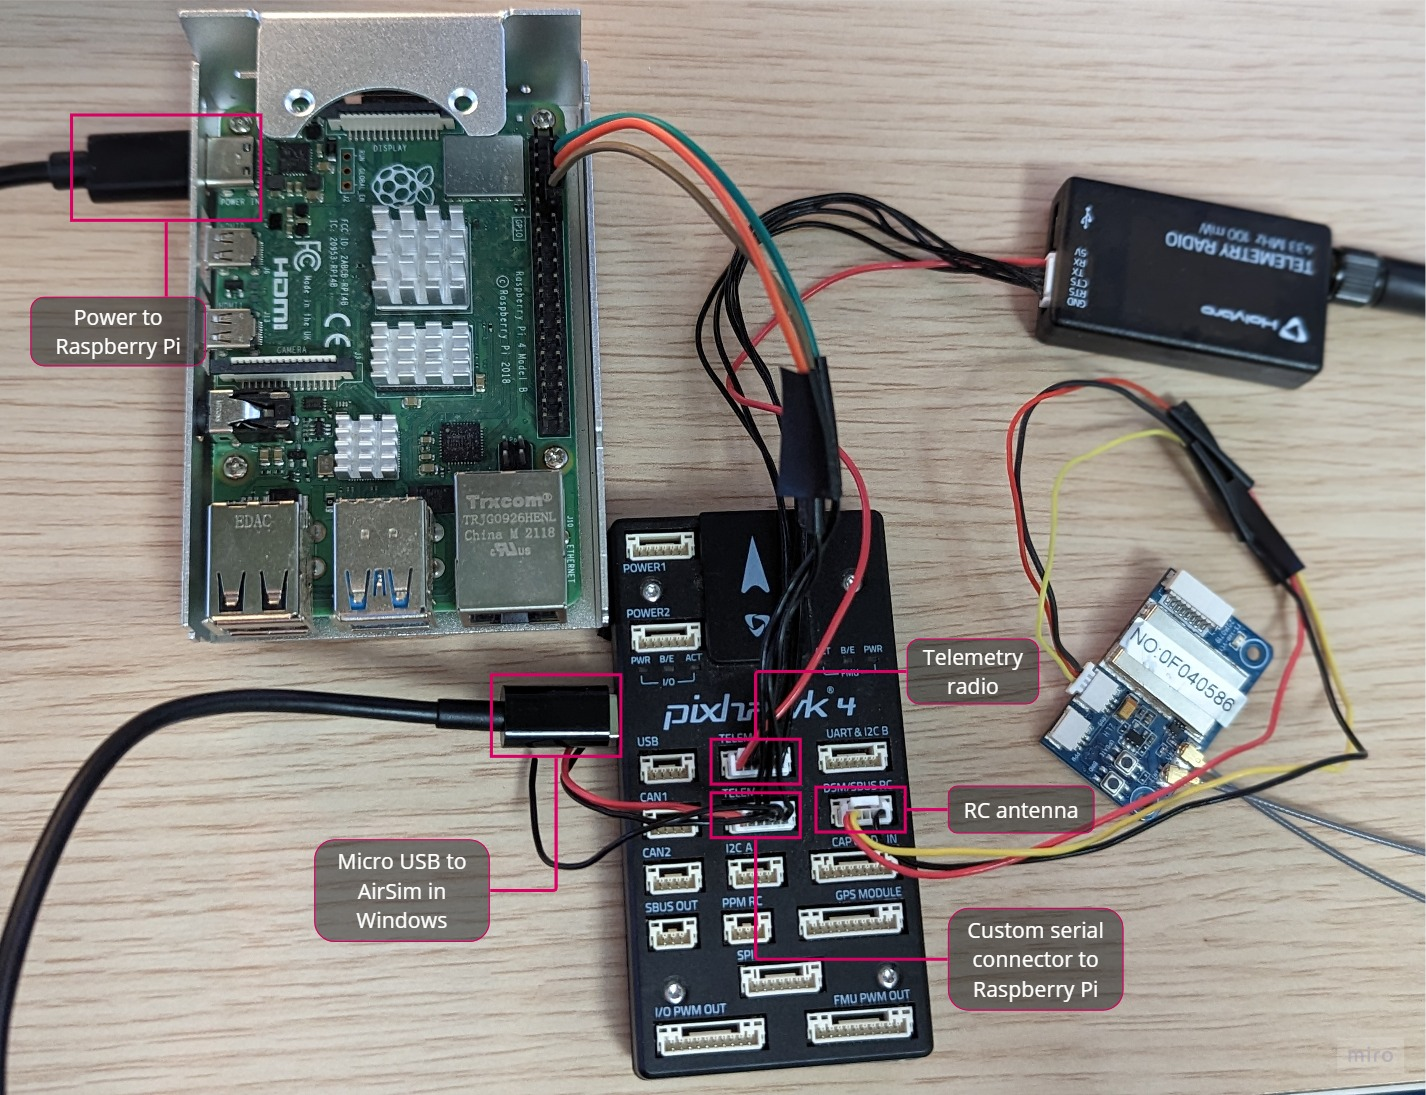
\includegraphics[width=\textwidth, keepaspectratio]{img/hitl-setup-picture.jpg}
  \caption{Pixhawk 4 board connected to the Raspberry Pi running the dronecontrol application and the Windows computer running the AirSim simulator, with telemetry radio for QGroundControl and RC receiver for manual control}
  \label{fig:hitl-setup-picture}
\end{figure}

After all the necessary connections are set up, the program can be started with the following command:
\mintinline{bash}{python -m dronecontrol follow --sim --serial COM[X]:57600}, where the exact COM port will vary depending on the particular USB port to which the telemetry radio is connected.


\subsection{PX4 HITL validation with Raspberry Pi}
\label{sec:test-5-rpi}

% Setup:    Raspberry Pi installation, RPi-Pixhawk connection
% Test:     - AirSim + follow on RPi + Pixhawk
%           - Serial connection
% Results:  wiring, performance metrics

The next step in the transition from a fully simulated environment to real flight is to connect the future onboard computer, the Raspberry Pi 4, to the Pixhawk flight controller and proceed with more realistic tests on the exact hardware that will be controlling the drone.
The main characteristics of the Raspberry Pi that have to be ensured to be able to progress further towards autonomous flight are:
\begin{enumerate}
    \item Capacity to function when power is provided from a battery
    \item Stability of serial connection to the Pixhawk board
    \item Ability to run the dronecontrol application and all its dependencies
    \item Connection to an external camera
    \item Performance of the computer vision algorithms with reduced processing power
\end{enumerate}

% installation
% xrdp
% battery tests

The complete installation process of all the required libraries and dependencies for the Raspberry Pi is explained in appendix \ref{app:install-dronecontrol-rpi}.
The most convenient method of controlling the small computer is through a remote desktop connection, where the screen contents and mouse and keyboard input are transmitted through a local network.
This way, accessing the Pi's desktop from the ground station computer is possible even during flight.
One option to achieve this is XRDP\footnote{\url{http://xrdp.org/}}, an open-source implementation of a Microsoft Remote Desktop Protocol server compatible with the Raspberry OS.

The first hardware connection to test is the power supply to the Raspberry.
As detailed in section \ref{subsec:onboard}, the selected method for powering the companion computer in the onboard configuration is through a secondary battery.
The connection will be made with a USB to USB-C cable from the battery to the Raspberry Pi.
The intent behind testing the power supply at this point in this process is to verify that it will be suitable for its purpose before it is actually needed to power the computer onboard the vehicle.
This power source must provide enough power to both maintain the processor running at an appropriate speed and provide power to the external camera in turn, which will be attached to the Pi's board and extract power from it.

A similar connector provides a channel for the Mavlink communication between the flight controller and the onboard computer.
In this case, one end of the connector is attached to the \texttt{TELEM2} port in the board and the TX/RX pins are attached to the UART pins on the Raspberry's GPIO header.
For this serial connection to work, both the flight controller and the companion computer need some additional configuration.
The Pixhawk needs to be configured through QGroundControl to enable a secondary Mavlink channel as, by default, only the \texttt{TELEM1} port used by the telemetry radio is configured.
The necessary parameters to modify and their values are collected in table \ref{tab:telem2-params}.
On the Raspberry side, the serial port comes configured to be used as a terminal instead of as a hardware serial port.
This can be fixed through the \texttt{raspi-config} command-line utility with the following steps: Interface options -> Serial Port -> Disable login shell, enable serial port hardware.
After that, the \texttt{/dev/serial0} address can be used to communicate to the device attached to the UART pins at the baudrate configured through QGroundControl.
The \texttt{raspi-config} tool and the connector used between the flight controller and the companion computer are shown in figure \ref{fig:serial-connection}.

\begin{table}[h!]
 \begin{center}
  \begin{tabular}{l|l}
    Parameter name & Value \\ \hline
    MAV\_1\_CONFIG & TELEM2 \\
    SER\_TEL2\_BAUD & 921600 \\
  \end{tabular}
  \caption{PX4 parameters that need to be configured to enable Mavlink communication through the secondary telemetry port}
  \label{tab:telem2-params}
 \end{center}
\end{table}


\begin{figure}
  \centering
  \makebox[\textwidth][c]{
  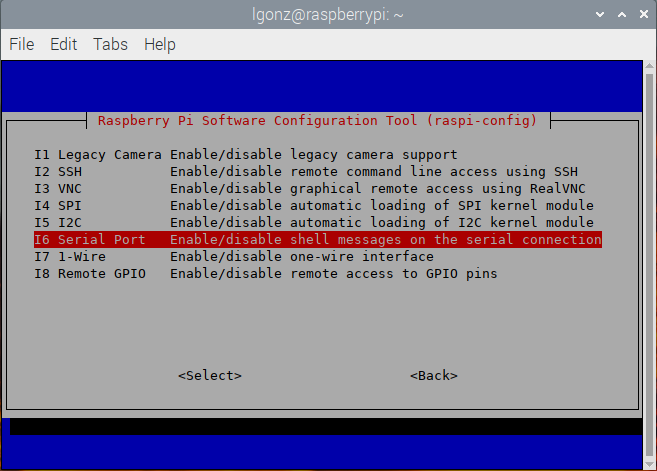
\includegraphics[width=.615\textwidth, keepaspectratio]{img/raspi-config.png}
  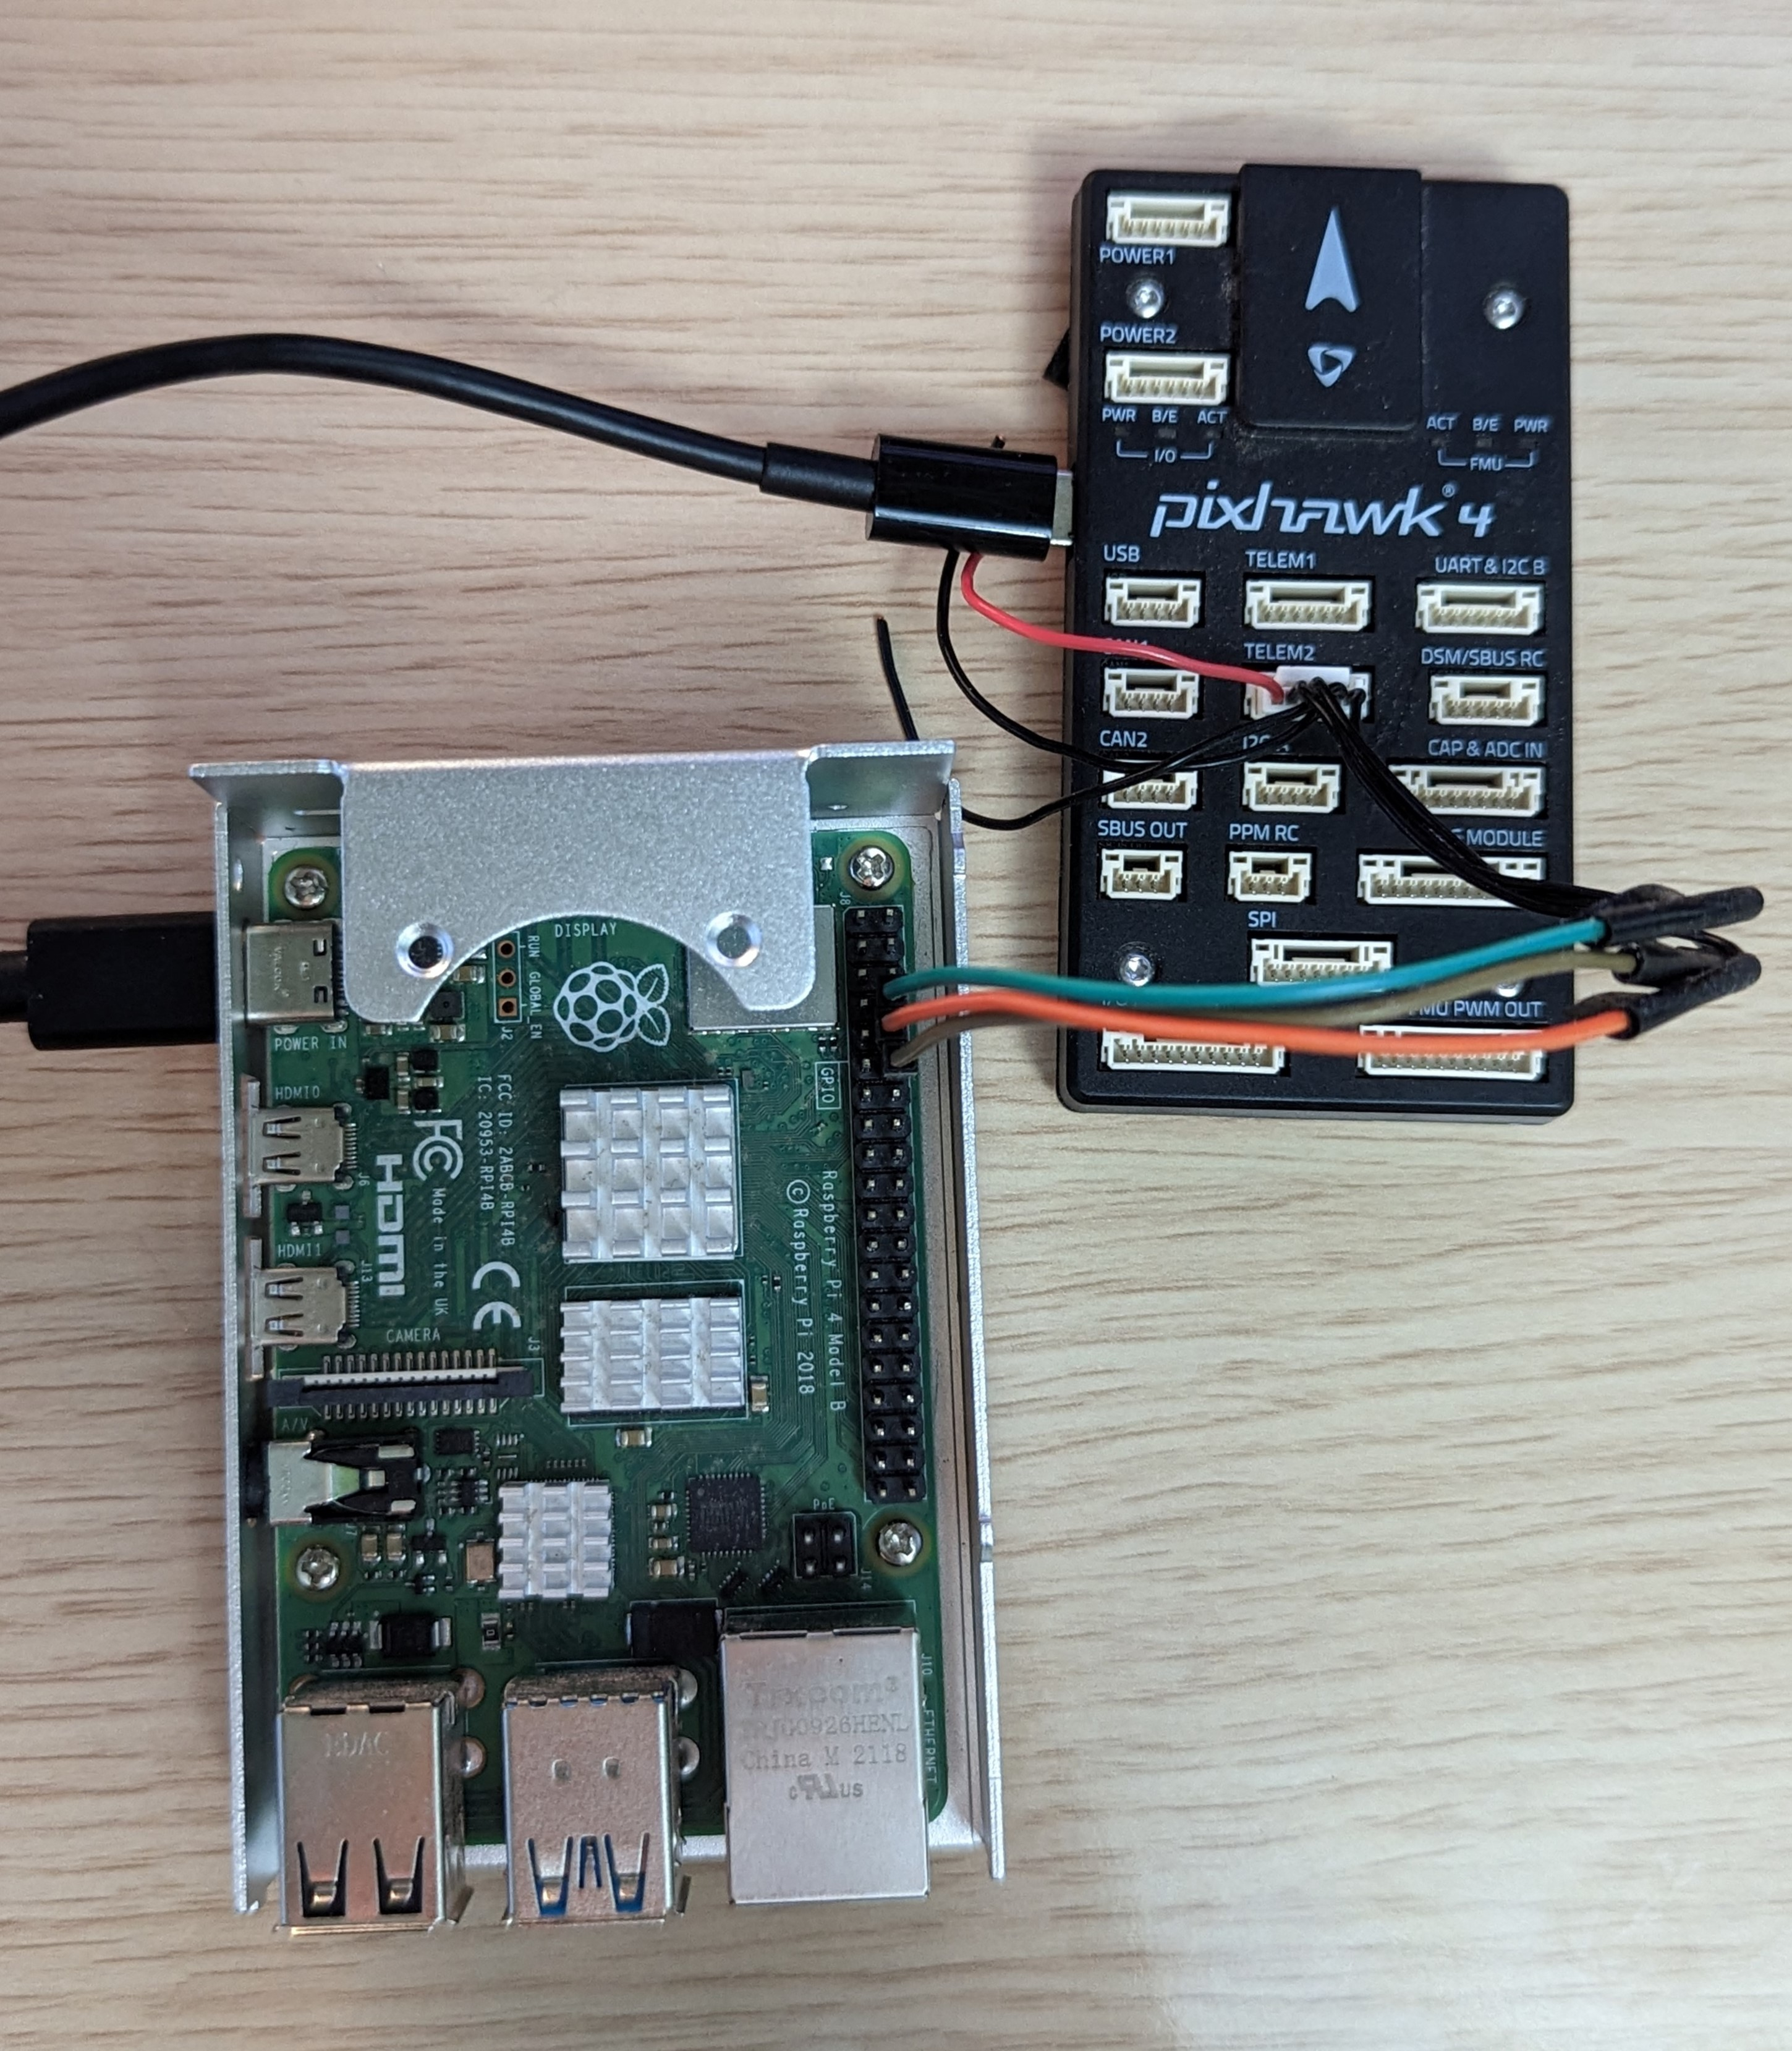
\includegraphics[width=.385\textwidth, keepaspectratio]{img/rpi-pixhawk-serial.jpg}}
  \caption{a) Picture of Raspberry's \texttt{raspi-config} and b) close-up of Pixhawk to Pi cable connection}
  \label{fig:serial-connection}
\end{figure}

The test camera utility will be used to validate this configuration.
At this point, the only physical connection to the ground station running AirSim or QGroundControl is through the development-only micro-USB port in the Pixhawk.
The results from running: \\
\begin{listing}[h!]
    \begin{minted}[breaklines, fontsize=\footnotesize, baselinestretch=1]{bash}
dronecontrol tools test-camera --hardware /dev/serial0:921600 --sim <AirSim host IP> --pose-detection
    \end{minted}
\end{listing}\\
can be seen on figure \ref{fig:rpi-airsim-test}.
On the right side, the remote connection to the Raspberry's desktop shows the output of the dronecontrol program running the pose detection algorithm on the images received from the simulator.
On the left side, the AirSim simulator shows the vehicle's movements as it reacts to the input from the flight controller and the companion computer.

\begin{figure}
  \centering
  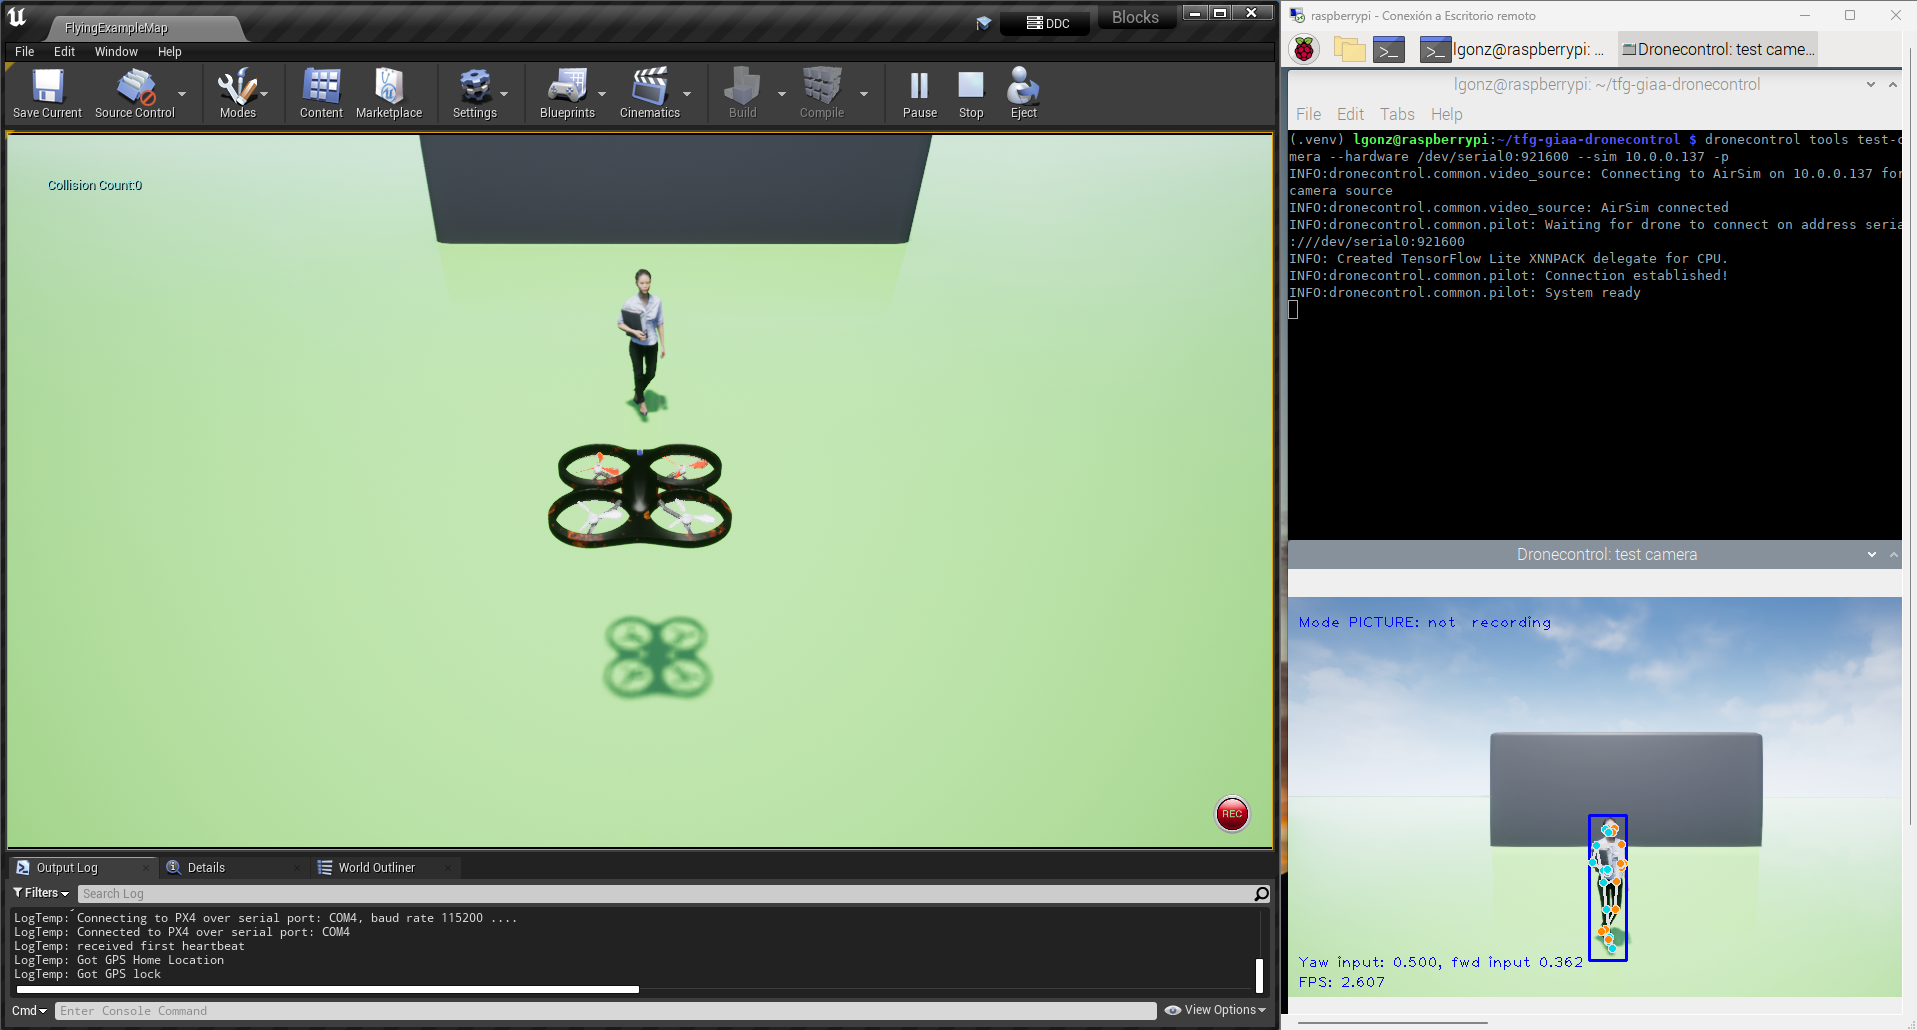
\includegraphics[width=\textwidth, keepaspectratio]{img/airsim-rpi-test.png}
  \caption{Left: AirSim simulator on Windows host, right: RPi desktop with Dronecontrol application and pose output}
  \label{fig:rpi-airsim-test}
\end{figure}

\subsection{Performance analysis}
\label{subsec:performance}

The main question left to answer before the vehicle can take to the air with this hardware and software is whether the less powerful processor in the Raspberry Pi 4b, a quad-core ARM Cortex-A72 64-bit SoC running at 1.5GHz, can handle the detection and tracking algorithms with enough performance to get similar results to those obtained with simulated hardware and achieve good reactions to real-time movement.
To do that, the average time that the program spends on each task in the running loop can be calculated and analyzed for different scenarios.
Then it will be possible to estimate the maximum speed at which the person being followed by the algorithm can move.

% Make sure there's a good loop diagram in that section pointed below, and that the enumerated parts are explained in detail
% Match numbers to added figures
From the follow loop presented in section \ref{sec:follow}, it is possible to divide the processing cost into several areas that can be measured independently: image processing, offboard control, manual input, and released thread (sleep).

\begin{figure}
  \centering
  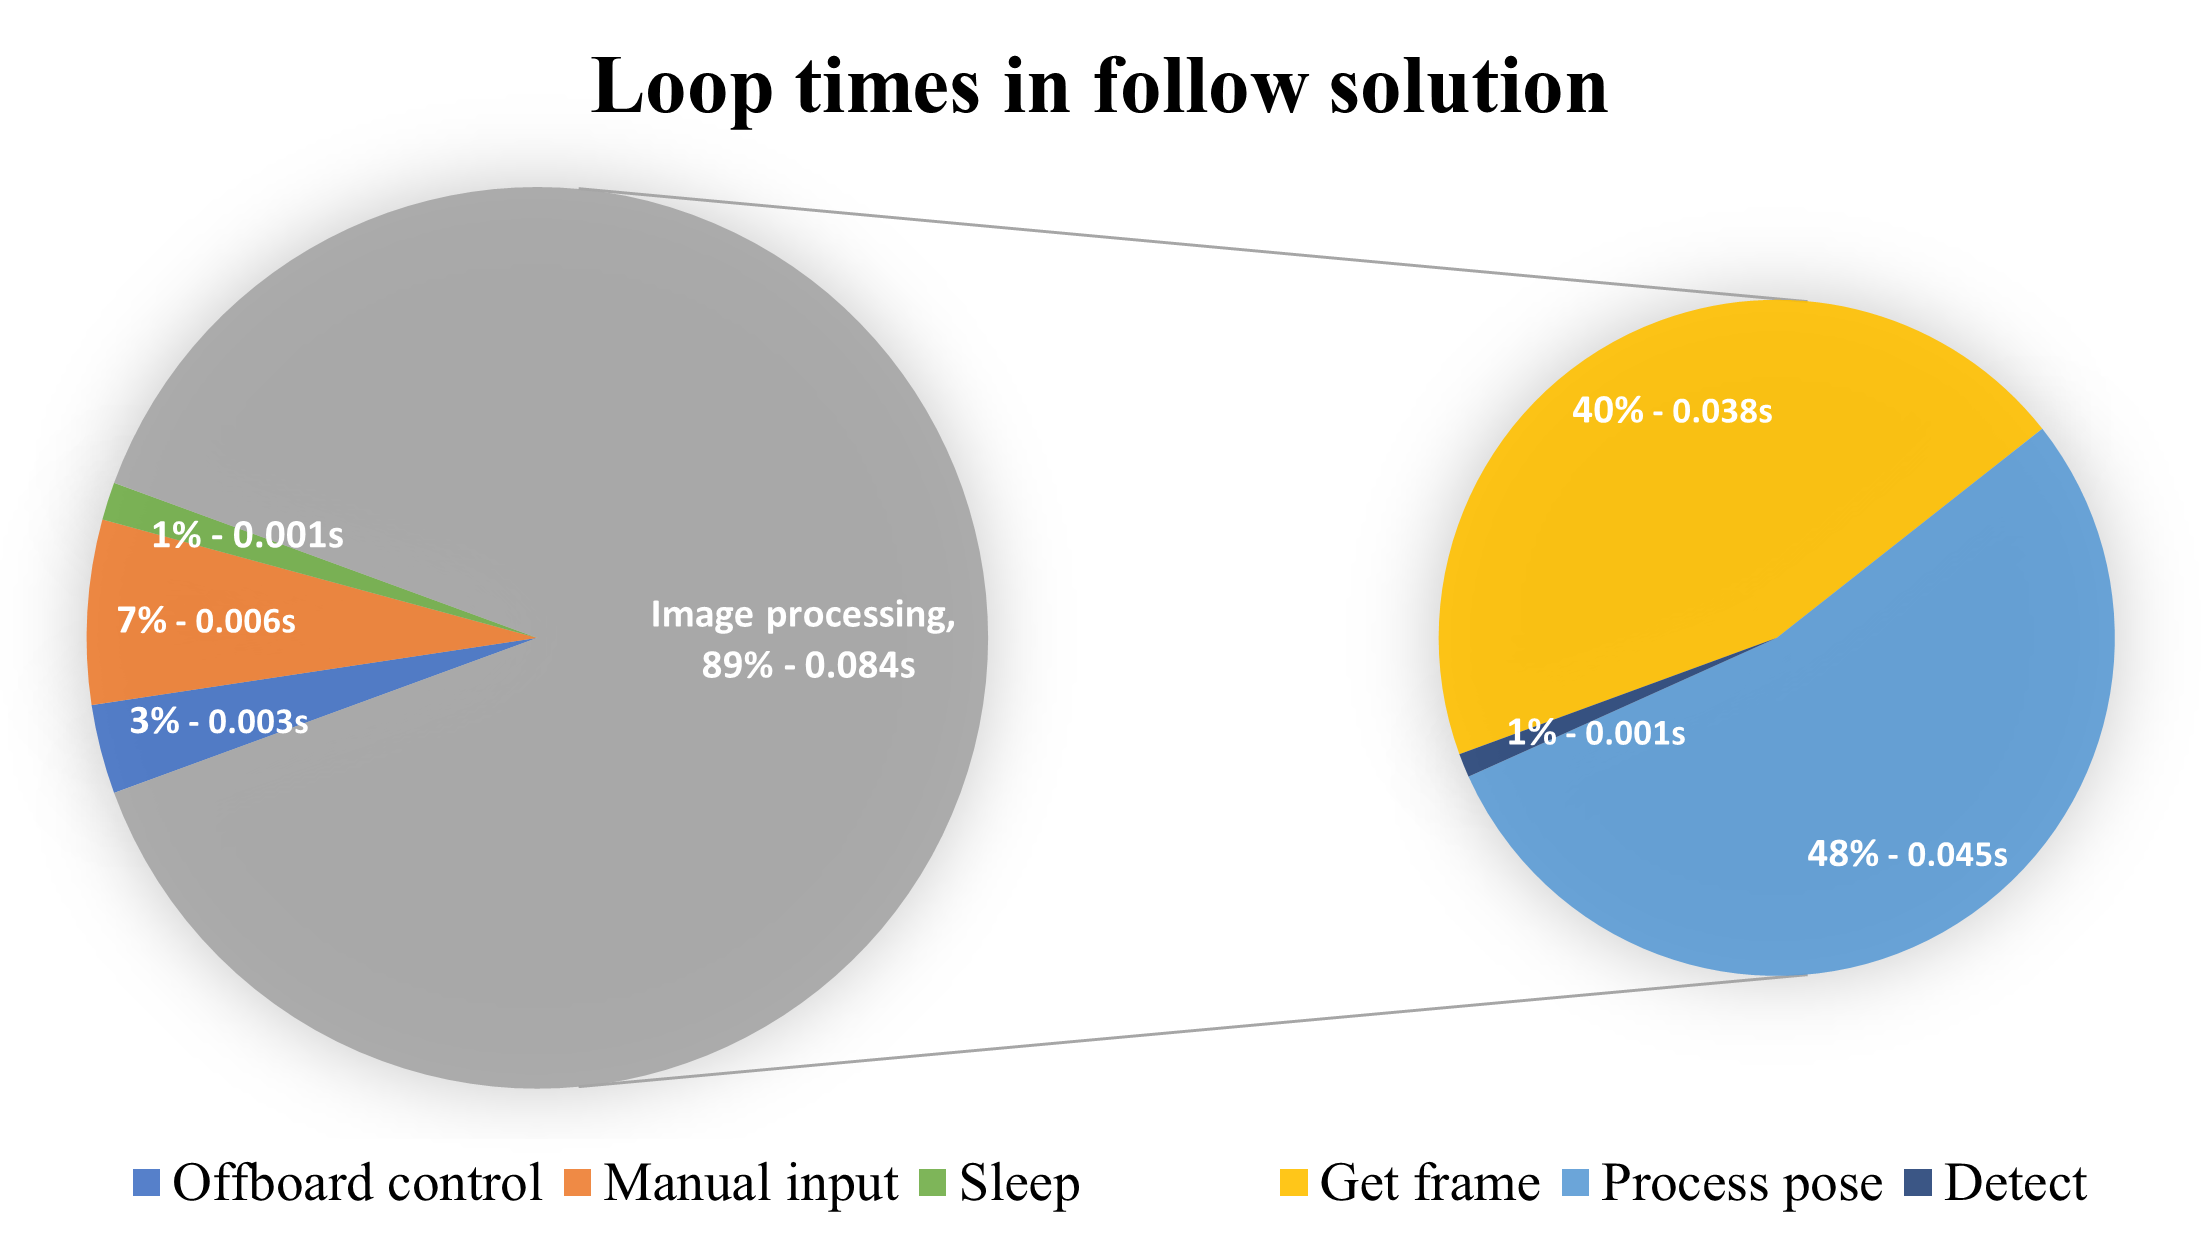
\includegraphics[width=.9\textwidth, keepaspectratio]{img/sitl-performance.png}
  \caption{Average percentages of a loop spent by each task in the follow solution with their corresponding average absolute times in seconds.}
  \label{fig:perf-sitl-sim}
\end{figure}

Figure \ref{fig:perf-sitl-sim} shows the time used for each task on an average run of the follow solution with simulated hardware (PX4 running in SITL mode with AirSim).
The time measurements have been taken by calculating the time difference between each statement's start and end and averaging across every iteration of the main loop.
The main cost in time of each execution is found in the image processing task, which takes around 89\% of the total loop time to run.
This is where the most significant differences in performance will come from between the simulated hardware and the solution running in the Pixhawk 4 + Raspberry Pi combination.
This image analysis process can be further subdivided to get a finer degree of control over how much time each part takes.
The three subtasks that makeup image processing are:
\begin{enumerate}
    \item Get frame: request a new frame from the video source.
    \item Process pose: send the frame to MediaPipe library for detection and tracking.
    \item Detect: calculate bounding box coordinates and define whether it is a valid pose.
\end{enumerate}

This further division is also shown in figure \ref{fig:perf-sitl-sim}, with each of these subtasks taking 40\%, 48\%, and 1\% of the total image processing time, respectively.
The total average time for each run of the follow loop is then 0.094 seconds, which results in an average performance of 10.5 FPS (frames-per-second).

Similar measurements have been taken for hardware combinations with different degrees of simulation, running the follow solution with offboard mode enabled and connected to the AirSim simulator.
These are:
\begin{enumerate}
    \item All simulated hardware: PX4 on SITL mode + dronecontrol on standalone computer + images from AirSim simulator video source.
    \item Simulated hardware with real images: PX4 on SITL mode + dronecontrol on standalone computer + images from the attached camera as video source.
    \item Test hardware with AC power supply: PX4 on HITL mode on Pixhawk 4 + dronecontrol on Raspberry Pi + images from the attached camera as video source.
    \item Test hardware with battery: PX4 on HITL mode on Pixhawk 4 + dronecontrol on Raspberry Pi powered by battery + images from the attached camera as video source.
\end{enumerate}


\begin{figure}
  \centering
  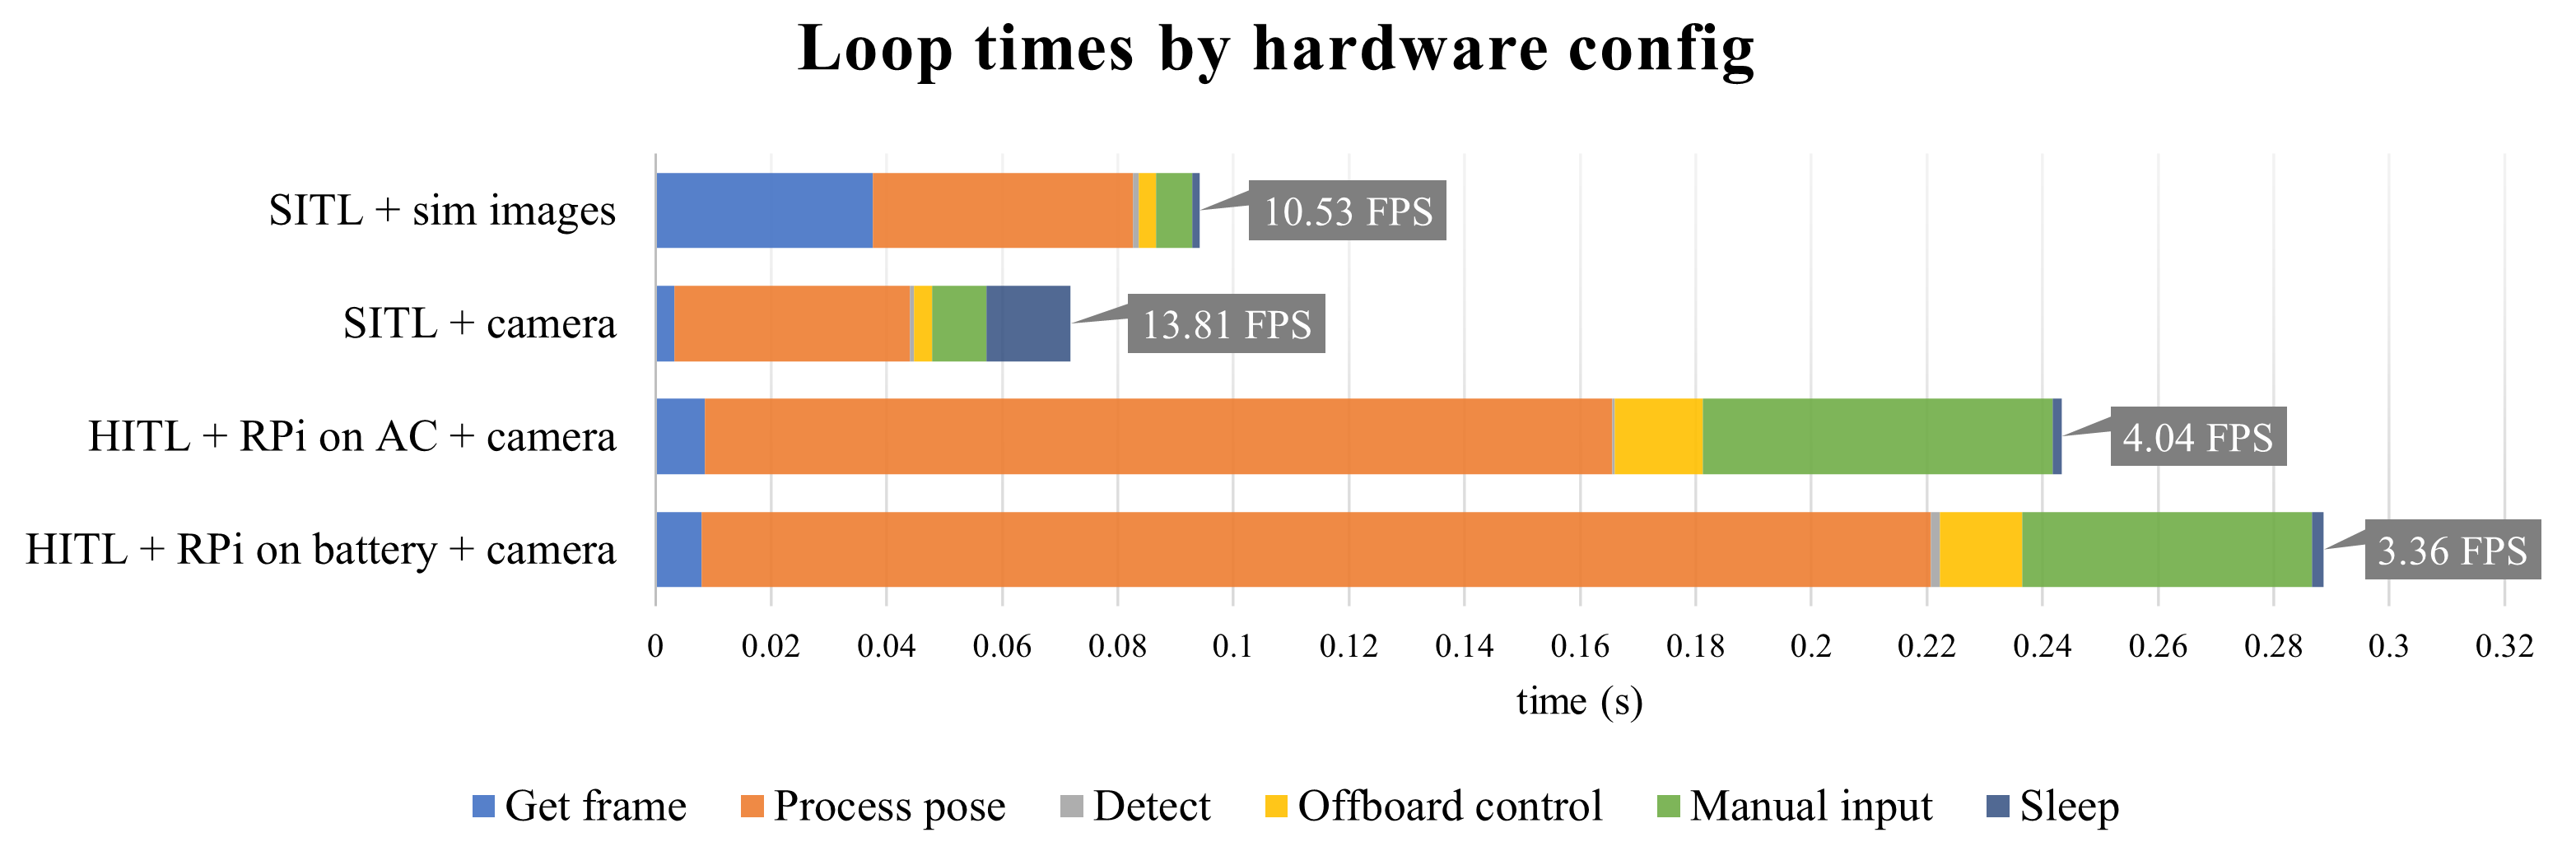
\includegraphics[width=\textwidth, keepaspectratio]{img/performance-graph.png}
  \caption{Average FPS and time spent on each task per iteration of the follow solution for the different hardware configurations.}
  \label{fig:perf-analysis}
\end{figure}


Figure \ref{fig:perf-analysis} shows the averages of the measurements taken for all the hardware combinations analyzed.
In the first test, it can be observed that the retrieval of each new frame from the AirSim simulator takes a much longer time than when an external camera is used.
This is because the simulation running on Unreal Engine is also limited in performance to what the computer can offer, which is not a cost that will be reflected when the simulation engine is no longer needed.
In the second test, the images from the simulator are replaced with the feed from an external camera connected to the computer. 
This results in a much lower cost for image retrieval and the best performance of any of the tests, with an average of 14 FPS and peaks of more than 20 FPS.
For the third and fourth tests, the image-processing calculations are moved to the onboard Raspberry Pi computer, which increases the time needed for pose-processing by one order of magnitude.
There is also a noticeable difference in performance in the Raspberry's processor between powering the computer through the AC power supply and through an external battery, stemming from the fact that the former supplies 3A of current to the board and the latter only 2A.

With these measurements, it is possible to understand how the board will behave during actual flight, with the last test being the closest to the expected flight conditions.
It should therefore be possible to sustain a performance of around 3 FPS during flight.
With a time between frames of around 0.3 seconds, and since the field of view of the camera used for flight tests is about four meters wide, the person being followed should be able to move at a speed of 3-4 m/s and remain within the view of the drone.


%% NICE TO HAVE:
%% Keyboard control actor in unreal that can walk around at a set speed
%% and be followed
%% EVEN NICER TO HAVE:
%% Web build of unreal project running dronecontrol
\section{Quadcopter flight tests}

Once the performance and safety of the control algorithms has been validated in the simulated environment, it is possible to begin flight tests and take to the air with a physical drone.
In this final section of the validation process, all the previous parts are put together in order to test how the developed software will perform in a real quadcopter during flight.
To do this, first it will be necessary to be build the base vehicle from its development kit and then integrate all the additional pieces needed for this project, like the companion computer and the camera.
Then, after making sure that the vehicle can fly with all the payload through remote control, both of the developed solutions will be tested:
first the hand-control solutions to verify that the autopilot can receive flight commands from an offboard computer and second the follow solution to verify that the companion computer can function as well during flight with its dedicated power supply as it did when it was stationary.

The exact steps that will be executed one after the other to ensure that safety is maintained during the whole process are as follows:

\begin{enumerate}
    \item Build the quadcopter with its basic components.
    \item Add custom payload.
    \item Fly with remote control and factory autopilot only, monitoring through QGroundControl.
    \item Fly with custom software from offboard computer with \texttt{test-camera} tool (\ref{subsec:cam-tool}).
    \item Fly with \texttt{test-camera} tool from onboard computer.
    \item Fly with custom hand-gesture control solution from offboard computer.
    \item Fly with custom follow solution from onboard computer.
\end{enumerate}

\subsection{Build process}
\label{sec:test-7-builddrone}

% Setup:    build drone, configuration, calibration
% Test:     - RC, GPS, 
%           - Arm, takeoff commands
%           - Camera holder
% Results:  wiring, drone pictures, QGroundControl calibration screens
%           holder 3d, drone close-up, camera feed


As has been mentioned before, the vehicle used in this project is the Holybro X500, designed specifically to work with PX4.
The detailed instructions to build the vehicle from its Development Kit can be found in the PX4 documentation \footnote{\url{https://docs.px4.io/main/en/frames_multicopter/holybro_x500_pixhawk4.html}}.
Figure \ref{fig:x500-dev-kit} shows all the parts that make up the complete vehicle.

\begin{figure}
  \centering
  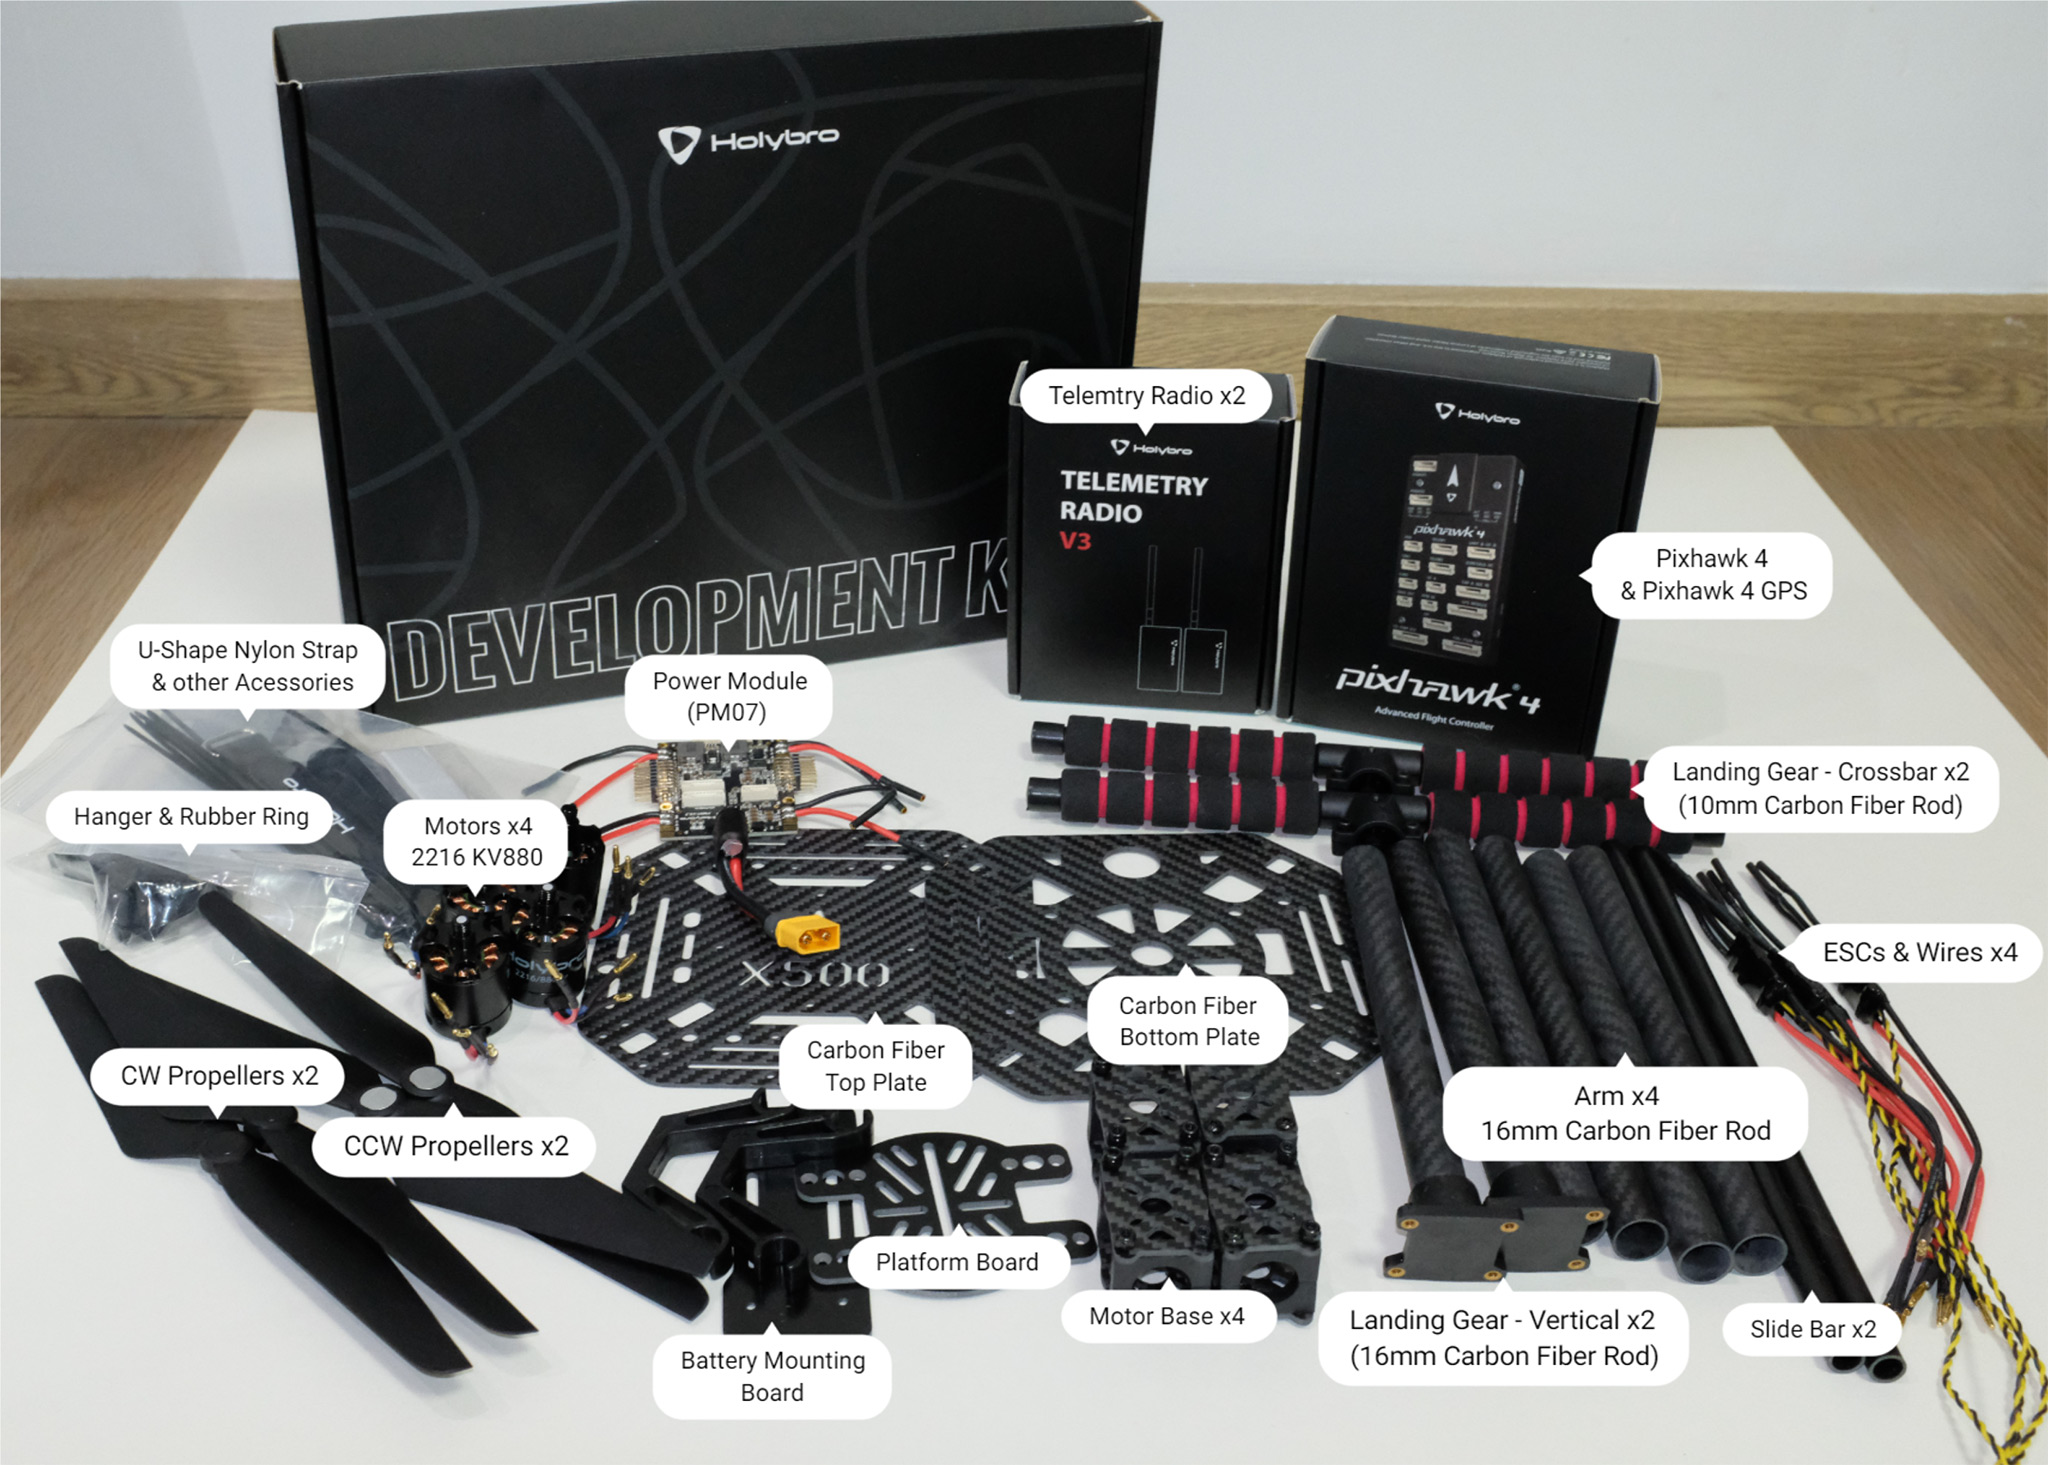
\includegraphics[width=.6\textwidth, keepaspectratio]{img/x500-dev-kit.jpg}
  \caption{Development kit for the Holybro X500.}
  \source{Adapted from \citetitle{px4-guide} \cite{px4-guide}.}
  \label{fig:x500-dev-kit}
\end{figure}


After all the standard parts are put together, the custom additions can be attached as well, using the remaining space in the frame.
The Raspberry Pi companion computer will sit just behind the autopilot to counterbalance the more weighted front of the vehicle where the GPS antenna is located.
This location also allows an easy connection between the autopilot and Raspberry's I/O pins with short cables, so as not to clutter the frame with wires excessively.

While in flight, the Raspberry Pi will be powered through a dedicated external battery that outputs power through a 2-ampere USB port.
This port will be connected with the Raspberry Pi's original power cable to its USB-C power supply socket.
As detailed in \ref{sec:test-5-rpi}, this current is enough to power the connected camera and run the developed software with acceptable performance.
This battery will be located underneath the autopilot, centered in the frame of the vehicle, so its weight destabilizes it as little as possible, as can be seen in figure \ref{fig:full-build}.

The camera also needs to be attached to the frame of the vehicle in a secure way, with the custom support described in section \ref{subsec:onboard}.
The holder attaches to the slide bars underneath the main frame of the vehicle so that the camera and its substantial weight are situated as close to the center of mass as possible behind the GPS platform.
The battery powering the engines and the autopilot, which is located on the underside of the carbon frame, is also moved slightly backward from its centered position to make space for the camera and compensate for its weight in the front.
Figure \ref{fig:camera-holder-closeup} shows how the underside of the vehicle looks with the camera attached.

\begin{figure}
  \centering
  
\includegraphics[width=0.8\textwidth, keepaspectratio]{img/placeholder.png}
  \caption{Complete build of the quadcopter with the main components highlighted}\label{fig:full-build}
\end{figure}
\todo[inline]{Figure \ref{fig:full-build}: take picture of complete build and annotate with arrows}

\begin{figure}
  \centering
  
\includegraphics[width=0.8\textwidth, keepaspectratio]{img/placeholder.png}
  \caption{Underside of the vehicle, with supports holding the main battery and the camera in place}
  \label{fig:camera-holder-closeup}
\end{figure}
\todo[inline]{Figure \ref{fig:camera-holder-closeup}: take picture of underside showing battery and camera holder}


After the vehicle has been built, there are additional installation and calibration steps that must be carried out before it can fly, also contained in the guide mentioned above.
Any simulation modes previously activated for testing must be deactivated from the Safety section of the vehicle configuration and the \texttt{MAV\_1\_CONFIG} parameter set to \texttt{TELEM2}, as described in section \ref{subsec:offboard}.
Then all the different sensors present, both embedded on the flight controller board and attached to the outside frame, need to be calibrated for this particular build.
The QGroundControl \ref{subsec:qgc} ground station application contains a configuration screen with all the calibration tools needed for the vehicle setup, shown in figure \ref{fig:qgc-config}.
The vehicle can be configured either by connecting the flight controller directly to the computer via the micro-USB port on its side or through a wireless connection by plugging the companion telemetry radio into the computer running QGroundControl.


\begin{figure}
  \centering
  
\includegraphics[width=\textwidth, keepaspectratio]{img/placeholder.png}
  \caption{Screenshot from the QGroundControl calibration and setup tools used to configure the vehicle}\label{fig:qgc-config}
\end{figure}
\todo[inline]{Figure \ref{fig:qgc-config}: take screenshot of sensor config in qgc}


\subsection{Initial tests}
\label{sec:test-8-flight}

% Setup:    flight plan
% Test:     - assisted takeoff, fly with RC
%           - tools/test_camera + record video
% Results:  video of flying, adjust pid set-point

\subsubsection{Baseline flight with factory software}
\label{subsec:fl-test-1}

Once the vehicle is fully configured, the RC controller and QGroundControl can be used to test assisted take-off and landing.
At this point, the drone should be able to maintain stable flight while using autopilot-assisted flight modes like Position Mode, where the roll and pitch sticks control the acceleration over the ground of the vehicle in the forward/backward and left/right directions relative to the heading the vehicle is facing.
The throttle controls the speed of ascent and descent. 
With the sticks centered, the vehicle will actively remain locked to a position in 3D space, compensating for wind and other forces.
This is the safest manual mode to test that the standard autopilot works as expected.

Through QGroundControl it is possible to map the different switches in the RC controller to different autopilot commands.
For this test, one of the switches with two positions will be mapped to arm/disarm, which controls whether the engines of the quadcopter can start or not; and one of the switches with three positions will be mapped to the landing/takeoff/position flight modes respectively, so the main autopilot modes can be tested by moving the switch between the available positions during flight.
This configuration exhausts all the channels available in the RC controller employed.
Other flight modes can be set by using the QGroundControl interface directly.

To carry out the flight, first, the main battery is connected to the socket in the power module.
This starts up the autopilot, the GPS antenna, the telemetry radio, and the RC receiver.
Afterward, QGroundControl can be started on a computer that has been connected to the second telemetry radio via USB.
If everything has worked correctly, the ground station application will automatically connect to the vehicle and situate its position on a satellite map.
Turning on the RC controller will likewise make it connect to the vehicle, as long as it has been paired correctly, as indicated in the guide linked in the first step of the build process.
Once all the wireless connections have been established, the drone can take off by first switching to the armed state and then switching to the takeoff flight mode.
While the drone is in the air, switching to the position flight mode will allow direct control through the joysticks in the controller.
Figure \ref{fig:flight-test-basic} shows an image from a flight carried out following these steps.
The full video of the test can be seen here.
%%%% [HERE] %%%%

\todo[inline]{Figure \ref{fig:flight-test-basic}: record video of flight test with RC control (+screenshot for text)}

\begin{figure}
  \centering
  
\includegraphics[width=.6\textwidth, keepaspectratio]{img/placeholder.png}
  \caption{Picture from flight tests}
  \label{fig:flight-test-basic}
\end{figure}

\subsubsection{Offboard computer flight with test tool}
\label{subsec:fl-test-2}

The second test flight will aim to make sure that the custom software can send takeoff and landing commands through a wireless MAVlink channel from the offboard computer (by using the telemetry radio through the developed test tool).
For this flight, the QGroundControl application cannot be connected to the vehicle since the telemetry radio channel will be blocked by the dronecontrol application.
The RC controller will therefore be used as a backup in case anything goes wrong with the software.
At any moment, the controller can switch flight mode and override the input generated from the dronecontrol application, recovering manual control.
Since the dronecontrol application can now easily arm the vehicle on its own while sending a takeoff command,
the two-way switch of the controller will be mapped for all the tests going forward to the command to kill the power to the engines.
This command could be helpful in edge cases to protect the vehicle or the surrounding area if the autopilot were to destabilize during takeoff and landing or completely lose control over the vehicle.
Now, once the main battery is connected again to the power module, the test tool is run with the following command for a Windows or a Linux machine, respectively:
\begin{minted}[breaklines, fontsize=\footnotesize, baselinestretch=1]{bash}
dronecontrol tools test-camera -r COM<X>:57600
\end{minted}
or
\begin{minted}[breaklines, fontsize=\footnotesize, baselinestretch=1]{bash}
dronecontrol tools test-camera -r /dev/ttyUSB0:57600
\end{minted}

After a successful connection to the vehicle, the T and L keys in the computer keyboard can be used for takeoff and landing, respectively, and the O key can be used to set the autopilot in offboard flight mode to make it able to receive velocity commands.
Afterward, the WASD keys can be used to control the forward and sideways velocity of the vehicle and the QE keys to control its yaw velocity.
Figure \ref{fig:flight-test-cam-offboard} displays the output on the terminal window of the computer, where the connection process and the sent velocity commands are shown, and the output on the camera from the offboard computer.

\begin{figure}
  \centering
  
\includegraphics[width=.45\textwidth, keepaspectratio]{img/placeholder.png}
  
\includegraphics[width=.45\textwidth, keepaspectratio]{img/placeholder.png}
  \caption{a) Terminal output from the \texttt{test-camera} tool running on an offboard computer, b) output from the camera of the offboard computer towards the vehicle in flight}
  \label{fig:flight-test-cam-offboard}
\end{figure}
\todo[inline]{Figure \ref{fig:flight-test-cam-offboard}: take screenshot from test-camera terminal and image output running for quadcopter + offboard companion computer}

\subsubsection{Onboard computer flight with test tool}
\label{subsec:fl-test-3}

The third and last test flight in this section will ensure that the custom software can send takeoff and landing commands through a cabled MAVlink channel from the onboard computer,
as well as making sure that the onboard camera can obtain a good image of the field of view of the vehicle during flight.
For that, the same tool will be used as in the last test, 
but in this instance, it will be run on the Raspberry Pi, and the connection will be established through the wired serial link between this onboard computer and the Pixhawk autopilot board.
Since the camera connected to the computer sending commands is now looking down on the pilot, it is possible to activate pose detection on the test images received from this onboard camera.
To start the flight test, the main battery and the secondary battery need to be attached, respectively, to the power module and to the Raspberry Pi.
After the onboard computer has started up, the easiest way to take control of it is with a remote desktop connection through WiFi, as explained in section \ref{sec:devenv}.
By this connection, a terminal window can be opened on the desktop, and the following command run:
\begin{minted}[breaklines, fontsize=\footnotesize, baselinestretch=1]{bash}
dronecontrol tools test-camera -r /dev/serial0:921600 -p
\end{minted}
As opposed to the flight using the telemetry radio, in this test the serial connection runs at a baudrate of 921600, which matches the configured baudrate on the \texttt{TELEM2} port of the Pixhawk board.
The "-p" option is used to enable pose detection in the output images.
The terminal and camera output can be seen in figure \ref{fig:flight-test-cam-onboard} and a video recording the remote desktop during the flight can be seen in here.
%%%% [HERE] %%%%


\begin{figure}
  \centering
  
\includegraphics[width=.6\textwidth, keepaspectratio]{img/placeholder.png}
  \caption{Pose detection algorithm running on images taken during flight}\label{fig:flight-test-cam-onboard}
\end{figure}
\todo[inline]{Figure \ref{fig:flight-test-cam-onboard}: record video of test-camera terminal and image output running for quadcopter + onboard companion computer (+ screenshot for text)}


\subsection{Hand gesture control}
\label{subsec:fl-test-4}

% Setup:    ...
% Test:     - Hand solution on windows through telemetry radio
%           - Free movement with offboard api
% Results:  video of flying, output from program

During basic flight tests, all the connections and individual parts of the software were validated in real flight.
Now it is time to integrate the piloting system with the image recognition results to test the vision-based control solutions developed.
The first solution to be used in flight will be the hand-gesture guidance system, as it is made to run on an offboard computer with more available processing resources and no dependence on battery-supplied power to work.
The setup will be identical to the second test flight (\ref{subsec:fl-test-2}) with the telemetry radio as the serial link and the onboard companion computer turned off
Once the autopilot board is powered up, the control solution can be started with the following command:
\begin{minted}[breaklines, fontsize=\footnotesize, baselinestretch=1]{bash}
dronecontrol hand -s <device>:57600
\end{minted}
where <device> is the COM port or TTY device the telemetry radio is attached to, depending on the platform.


After the pilot connects, the image from the webcam of the computer will appear on the screen with an outline over any detected hand.
To start controlling the vehicle, an open palm should be shown to the camera.
Then, a closed fist will make the drone take off, and pointing up with the index finger will start the offboard flight mode.
Afterward, moving the index finger right or left will make the vehicle mirror the movement, 
and moving the thumb right or left will make the vehicle move forward and backward, respectively.
At any point during the test, an open hand will make the vehicle land at its current place, and losing sight of the controlling hand will make the vehicle return to the starting position before landing as well

\todo[inline]{Figure \ref{fig:flight-test-hand-takeoff}, \ref{fig:flight-test-hand-right}, \ref{fig:flight-test-hand-fwd}: record video side-by-side computer screen with terminal and image output and video from vehicle flying, synced, hand solution on windows (+ 3 screenshots of different movements)}

\begin{figure}
  \centering
  
\includegraphics[width=.6\textwidth, keepaspectratio]{img/placeholder.png}
  \caption{Image taken during flight controlled by the hand-gesture solution. Vehicle is taking off}
  \label{fig:flight-test-hand-takeoff}
\end{figure}

\begin{figure}
  \centering
  
\includegraphics[width=.6\textwidth, keepaspectratio]{img/placeholder.png}
  \caption{Image taken during flight controlled by the hand-gesture solution. Vehicle is moving to the right.}\label{fig:flight-test-hand-right}
\end{figure}

\begin{figure}
  \centering
  
\includegraphics[width=.6\textwidth, keepaspectratio]{img/placeholder.png}
  \caption{Image taken during flight controlled by the hand-gesture solution. Vehicle is moving forward}\label{fig:flight-test-hand-fwd}
\end{figure}

\subsection{Target detecting, tracking and following}
\label{subsec:fl-test-5}

% Setup:    ...
% Test:     - Follow solution on RPi
%           - Controller response to real input
% Results:  video of flying, output from program

Finally, it only remains to test the follow control solution.
In this section, the companion computer will be running the follow program and it will be validated whether it is capable of keeping track of and following a moving target during a non-simulated flight.
The setup will be identical to the third test in section \ref{subsec:fl-test-3}, without needing a wireless telemetry connection.
The telemetry radio is, therefore, free to be used, for example, to track the vehicle's path through the QGroundControl application on a secondary, offboard computer.
The control application will be started with the following command:
\begin{minted}[breaklines, fontsize=\footnotesize, baselinestretch=1]{bash}
dronecontrol follow -s /dev/serial0:921600
\end{minted}
Figure \ref{fig:flight-test-follow} shows the process in the terminal of getting the vehicle to takeoff (T key), activating offboard flight mode (O key), and starting movement tracking of the detected figure.
The maximum frames per second managed by the program running on the Pi is around %______.
In practice, this means that the person being tracked by the drone has to move quite slowly for the camera not to lose sight of them before the autopilot can send the command to the vehicle to move to the previously detected position.
At the end of the program run, the average loop time and average runtime for each of the tasks in the main loop are shown in the terminal.
From the measures obtained for the test flight carried out, we can see %______________.
However, for a proof-of-concept scenario, this is an acceptable performance.
\todo[inline]{Write: Compare performance in follow flight to that in the HITL section}


\begin{figure}
  \centering
  
\includegraphics[width=.6\textwidth, keepaspectratio]{img/placeholder.png}
  \caption{Terminal and image output of the dronecontrol follow solution running on the Raspberry Pi}
  \label{fig:flight-test-follow}
\end{figure}

\todo[inline]{Figure \ref{fig:flight-test-follow}: same recording as hand solution (+ screenshot from terminal and image output)}


\clearpage